% Paper A: the author's structure (analysis -> nonlinear -> algorithm -> Bayesian layer -> results -> limits).
% Document class selection (\input as the first line of each main.tex).
% SIMODS is typeset with SIAM's online-journal class siamonline<date>.cls. The class is not on CTAN;
% download it from SIAM's author page (the CI tries to) and place it in paper/shared/siam/.
% Without it the paper builds with a compatible fallback (article + siamshim.tex), so that text,
% numbering and cross-references can be checked; the submission must use the official class.
\makeatletter
\let\pf@cls\relax
\IfFileExists{siamonline220329.cls}{\def\pf@cls{siamonline220329}}{}
\IfFileExists{siamonline250211.cls}{\def\pf@cls{siamonline250211}}{}
\ifx\pf@cls\relax
  \documentclass[11pt]{article}
  \def\paperclass{shim}
\else
  \edef\pf@doc{\noexpand\documentclass[review,onefignum,onetabnum]{\pf@cls}}
  \pf@doc
  \def\paperclass{siam}
\fi
\makeatother

% Common preamble of both papers (after docclass.tex).
\def\pfshimname{shim}
\ifx\paperclass\pfshimname
  % Fallback that mimics the parts of siamonline used by the papers (only when the class is absent).
\usepackage[letterpaper,margin=1.15in]{geometry}
\usepackage{amsmath,amssymb,amsthm}
\usepackage[T1]{fontenc}
\usepackage{lmodern}
\usepackage{fancyhdr}
\newcommand{\headers}[2]{\pagestyle{fancy}\fancyhf{}\fancyhead[LE]{\small\thepage\quad\textsc{#2}}%
  \fancyhead[RO]{\small\textsc{#1}\quad\thepage}\fancyhead[LO,RE]{}\renewcommand{\headrulewidth}{0pt}}
\newcommand{\email}[1]{\texttt{#1}}
\newcommand{\funding}[1]{\par\noindent\textbf{Funding:} #1}
\newenvironment{keywords}{\par\smallskip\noindent\textbf{Key words.}\ }{\par}
\newenvironment{MSCcodes}{\par\smallskip\noindent\textbf{MSC codes.}\ }{\par}
\newenvironment{AMS}{\par\smallskip\noindent\textbf{AMS subject classifications.}\ }{\par}
\renewenvironment{abstract}{\par\small\noindent\textbf{Abstract.}\ }{\par\normalsize}

\else
  \usepackage{amssymb}
  \newsiamremark{remark}{Remark}
  \newsiamremark{example}{Example}
  \newsiamthm{assumption}{Assumption}
\fi
\usepackage{mathtools}
\usepackage{graphicx}
\graphicspath{{../shared/figures/}}
\usepackage{booktabs,array,tabularx,multirow}
\usepackage[dvipsnames]{xcolor}
\usepackage{tikz}
\usetikzlibrary{arrows.meta,positioning,calc,fit,shapes.geometric,backgrounds}
\usepackage{algorithm}
\usepackage{algpseudocode}
\usepackage{enumitem}
\setlist{nosep,leftmargin=*}
\ifx\paperclass\pfshimname
  \usepackage[hidelinks]{hyperref}
  \usepackage[capitalize,nameinlink]{cleveref}
  % Fallback theorem environments (loaded after hyperref and cleveref so that names resolve).
\theoremstyle{plain}
\newtheorem{theorem}{Theorem}[section]
\newtheorem{lemma}[theorem]{Lemma}
\newtheorem{proposition}[theorem]{Proposition}
\newtheorem{corollary}[theorem]{Corollary}
\theoremstyle{definition}
\newtheorem{definition}[theorem]{Definition}
\newtheorem{assumption}[theorem]{Assumption}
\theoremstyle{remark}
\newtheorem{remark}[theorem]{Remark}
\newtheorem{example}[theorem]{Example}

\else
  \makeatletter\@ifpackageloaded{cleveref}{}{\usepackage[capitalize,nameinlink]{cleveref}}\makeatother
\fi
\crefname{assumption}{Assumption}{Assumptions}
\crefname{example}{Example}{Examples}
\crefname{remark}{Remark}{Remarks}
\crefname{algorithm}{Algorithm}{Algorithms}
% ---------------------------------------------------------------------------------------------
% Notation macros. ONE symbol, ONE meaning: every macro below is listed in the notation table
% (sections/notation.tex) and the script tools/check_notation.py checks the correspondence.
% ---------------------------------------------------------------------------------------------
% number sets and rings
\newcommand{\R}{\mathbb{R}}
\newcommand{\C}{\mathbb{C}}
\newcommand{\Z}{\mathbb{Z}}
\newcommand{\ring}{\mathcal{R}}            % ring of constant-coefficient operators C[d_t,d_x] = C[tau,xi]
% operators and their algebra
\DeclareMathOperator{\Ann}{Ann}             % annihilator ideal of a function
\DeclareMathOperator{\gcdop}{gcd}
\DeclareMathOperator{\spn}{span}
\DeclareMathOperator{\rank}{rank}
\DeclareMathOperator{\diag}{diag}
\DeclareMathOperator{\tr}{tr}
\newcommand{\Var}{V}                        % characteristic variety V(P)
\newcommand{\EP}{\mathrm{EP}}               % exponential-polynomials
\newcommand{\dd}{\,\mathrm{d}}
\newcommand{\Id}{\mathrm{Id}}
\newcommand{\Gu}{G_u}                       % intrinsic operator gcd Ann(u)
\newcommand{\Ju}{J_u}                       % cofactor ideal, Ann(u) = G_u J_u
\newcommand{\sigp}{\Sigma_{\mathrm p}}      % point spectrum V(J_u)
\newcommand{\sumop}{\mathcal{S}}            % sum operator (u_1,...,u_N) -> sum u_j
\newcommand{\Eint}{E_{\mathrm{int}}}        % interaction term
\newcommand{\flow}{\Phi}                    % flows Phi_n(t) = e^{t A_n}
\newcommand{\cF}{c_{F}}                     % Friedrichs cosine
\newcommand{\thetaF}{\theta_{F}}            % Friedrichs angle
\newcommand{\gN}{\gamma_{N}}                % conditioning constant of the sum operator
\newcommand{\deltaP}{\delta(P)}             % ambiguity dimension
\newcommand{\Hs}{H^{s}}                     % Sobolev space of index s
\newcommand{\noise}{\sigma_{n}}             % observation noise standard deviation
\newcommand{\sigbin}{\sigma_{\kappa}}       % noise standard deviation of one Fourier bin
\newcommand{\Nsamp}{N_{\mathrm s}}          % number of posterior field samples
\newcommand{\keff}{k_{\mathrm{eff}}}        % effective number of factors
\newcommand{\cloud}{W}                      % cloud of factor vectors (a weighted point measure)
\newcommand{\Mfit}{\mathsf{M}}              % a candidate structure (model)
\newcommand{\lab}[1]{\textsf{#1}}           % output labels
\newcommand{\FC}{\lab{FIT-COMPATIBLE}}
\newcommand{\IDK}{\lab{ID-KER}}
\newcommand{\MIS}{\lab{MISFIT}}
\newcommand{\UND}{\lab{UNDECIDED}}
\newcommand{\Normal}{\mathcal{N}}
\newcommand{\E}{\mathbb{E}}
\newcommand{\abs}[1]{\lvert#1\rvert}
\newcommand{\norm}[1]{\lVert#1\rVert}
\newcommand{\ip}[2]{\langle#1,#2\rangle}
% editorial
\newcommand{\roleinalg}[1]{\par\noindent\emph{Role in the algorithm.} #1\par}
\newcommand{\inbrief}[1]{\par\smallskip\noindent\emph{In brief.} #1\par\smallskip}



\title{Grouping Structure of Linear Partial Differential Equations\\and Its Use in Learning Them from Data}
\author{Flavio Pricoco\thanks{\email{flaflapr@gmail.com}}}
\headers{Grouping structure of PDEs in learning}{F. Pricoco}

\begin{document}
\maketitle

\begin{abstract}
In Fourier variables a linear partial differential equation with constant coefficients is a polynomial, and a
factorization of this polynomial splits every solution into groups of modes, one group per factor. We study this
grouping structure and use it to learn equations from noisy data. On the analytical side we show that the groups are
the factors of the symbol and not the additive terms of the operator, that the split is unique up to a
finite-dimensional overlap given by an intersection number, that its stability is governed by the conditioning of the
sum of the factors' solution spaces (for two factors, their Friedrichs angle), and that without a priori bounds finite
data can support but never certify an equation. On the algorithmic side we group twice: Fourier modes into factors
within one sample of the field, by fitting the curves of the dispersion relation, and factors across posterior samples,
by Dirichlet-process clustering. The output is a distribution over equations with intervals and labels stating what
the data support. On twenty random equations not used in development the method returns the right or an equivalent
equation on nineteen, fourteen of them with a confident label, and is never wrong without warning, while each of the
three library-regression baselines run on this set is wrong without warning on at least thirteen. On sixty grid inputs with
independent fields and noise it is always right, and on the ten-equation development benchmark, in three noise and
sampling designs, it recovers all thirty factor sets.
\end{abstract}

\begin{keywords}
equation discovery, partial differential equations, operator factorization, Friedrichs angle, matrix pencil,
Dirichlet process, uncertainty quantification
\end{keywords}

\begin{MSCcodes}
35E20, 62F15, 65M32, 68T05
\end{MSCcodes}

% Paper A: introduction (follows the author's outline).
\section{Introduction}\label{sec:intro}
A partial differential equation with constant coefficients becomes, in Fourier variables, a polynomial: the operator
$(\partial_t+c\,\partial_x)(\partial_t-\nu\,\partial_x^2)$ of a quantity that is carried by a flow and diffuses becomes
$(\tau+c\,\xi)(\tau-\nu\,\xi^2)$. Polynomials can be multiplied and factored, and a factorization of the symbol splits
every solution into pieces, one for each factor: here a travelling profile, whose Fourier modes lie on the line
$\lambda=-ic\kappa$, and a diffusing one, whose modes lie on the parabola $\lambda=-\nu\kappa^2$ (\cref{fig:branches}).
This paper is about that splitting, which we call the \emph{grouping structure} of the equation, and about how a
machine-learning algorithm can find it in noisy data and use it to recover the equation. The example matters in
practice: methods that regress $u_t$ on a library of terms look for a single sum of terms, and every one we tested
returns a wrong equation for it at $5\%$ noise, without warning.

% Shared figure for the introductions: the two groups of the running example as curves of modes.
\begin{figure}[tbp]
\centering
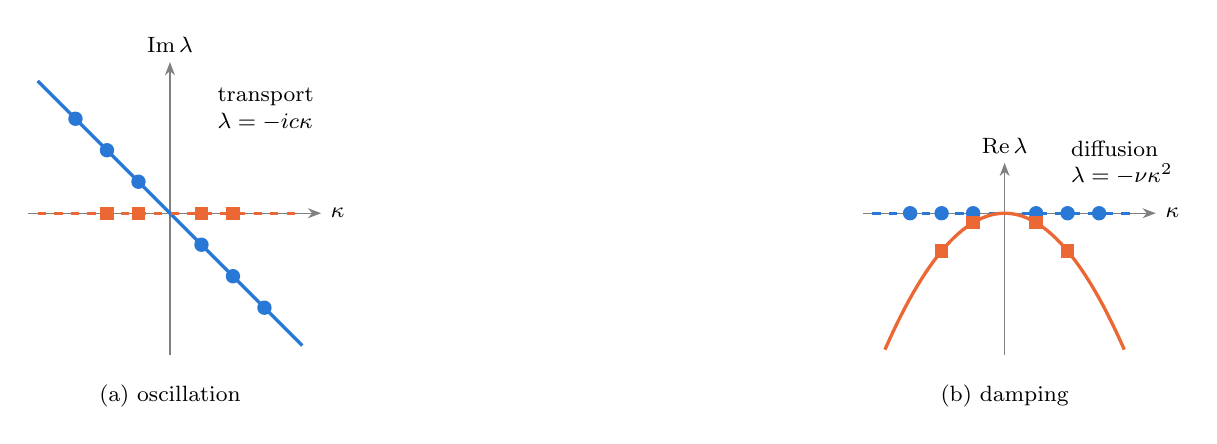
\begin{tikzpicture}[x=0.40cm,y=0.40cm,>=Stealth,font=\footnotesize]
  % (a) oscillation slice
  \begin{scope}
    \draw[->,gray] (-4.5,0)--(4.8,0) node[right,black]{$\kappa$};
    \draw[->,gray] (0,-4.5)--(0,4.8) node[above,black]{$\operatorname{Im}\lambda$};
    \draw[very thick,color={rgb,255:red,42;green,120;blue,214}] (-4.2,4.2)--(4.2,-4.2);
    \draw[very thick,color={rgb,255:red,235;green,104;blue,52},dashed] (-4.2,0)--(4.2,0);
    \foreach \k in {-3,-2,-1,1,2,3} \fill[color={rgb,255:red,42;green,120;blue,214}] (\k,-\k) circle (2.6pt);
    \foreach \k in {-2,-1,1,2} \fill[color={rgb,255:red,235;green,104;blue,52}] (\k,0) +(-2.4pt,-2.4pt) rectangle +(2.4pt,2.4pt);
    \node[anchor=west,align=left] at (1.2,3.3) {transport\\$\lambda=-ic\kappa$};
    \node at (0,-5.8) {(a) oscillation};
  \end{scope}
  % (b) damping slice
  \begin{scope}[xshift=10.6cm]
    \draw[->,gray] (-4.5,0)--(4.8,0) node[right,black]{$\kappa$};
    \draw[->,gray] (0,-4.5)--(0,1.6) node[above,black]{$\operatorname{Re}\lambda$};
    \draw[very thick,color={rgb,255:red,42;green,120;blue,214},dashed] (-4.2,0)--(4.2,0);
    \draw[very thick,color={rgb,255:red,235;green,104;blue,52},domain=-3.8:3.8,samples=60] plot (\x,{-0.3*\x*\x});
    \foreach \k in {-3,-2,-1,1,2,3} \fill[color={rgb,255:red,42;green,120;blue,214}] (\k,0) circle (2.6pt);
    \foreach \k in {-2,-1,1,2} \fill[color={rgb,255:red,235;green,104;blue,52}] (\k,{-0.3*\k*\k}) +(-2.4pt,-2.4pt) rectangle +(2.4pt,2.4pt);
    \node[anchor=west,align=left] at (1.8,1.6) {diffusion\\$\lambda=-\nu\kappa^2$};
    \node at (0,-5.8) {(b) damping};
  \end{scope}
\end{tikzpicture}
\caption{The idea of the paper on the equation $(\partial_t+c\,\partial_x)(\partial_t-\nu\,\partial_x^2)u=0$. Every Fourier mode
$e^{\lambda t+i\kappa x}$ of a solution lies on the zero set of one factor of the symbol $(\tau+c\xi)(\tau-\nu\xi^2)$: circles
on the line of the transport factor, squares on the parabola of the diffusion factor (schematic; \cref{fig:directions}
shows the modes found in noisy data). Learning the equation means learning these two groups.}\label{fig:branches}
\end{figure}


Two questions organize the work. The first is analytical: which pieces of an equation does a solution actually carry,
how uniquely, and how stably? The answer is that the pieces are the \emph{factors} of the symbol, not the additive
\emph{terms} of the operator; that the split is unique up to a finite-dimensional overlap whose dimension is an
intersection number; and that its stability is governed by the Friedrichs angle between the solution spaces of the
factors. The second question is algorithmic: how can one learn the groups from finitely many noisy observations, and
what should the output say about how well they were learned? Our answer is an algorithm that groups twice. Within one
sample of the field it groups Fourier modes into factors, using the fact that the modes of one factor lie on one curve
of the dispersion relation. Across posterior samples it groups the factors found in each sample into clusters, using a
Dirichlet-process mixture. The output is a distribution over equations with labels that say what the data can and
cannot support.

\paragraph{Contributions}
\begin{enumerate}
  \item An analytical account of the grouping structure: identification and uniqueness (\cref{thm:ident,prop:unique}),
  the factor decomposition with its exact ambiguity $\deltaP$ (\cref{thm:factor}), its conditioning
  (\cref{thm:hm}), and the impossibility of grouping by terms (\cref{prop:terms,prop:discont}).
  \item An algorithm that turns this structure into a learning procedure: interpolation with a sampling-based
  treatment of the high-frequency band, a matrix pencil per wavenumber, a joint grouping-and-fitting of the modes, and
  a Bayesian layer that groups factors across samples and attaches intervals whose empirical coverage is
  $0.94$ at nominal $0.90$.
  \item Evidence: on twenty random equations not used in development the method is right or equivalent on $19$
  ($14$ with a confident label, $5$ with an abstaining label and correct factors) and never wrong without warning,
  against $13$ or more such failures for each of the three library-regression baselines run on this set; on $60$ grid
  inputs with independent fields and noise it is always right, against $13$ silent failures for weak SINDy; on a
  benchmark of ten equations in three designs, on which its parameters were tuned, it recovers all $30$ factor
  sets, while the best library regression is right or equivalent on $25$ and wrong without warning on $5$.
\end{enumerate}

% Shared: relation to prior work (what is classical, what is new).
\paragraph{Relation to prior work}
Most methods that learn a PDE from data regress a time derivative on a library of candidate terms: SINDy and
PDE-FIND~\cite{BruProKut16,RudBruProKut17}, their weak, ensemble and Bayesian variants~\cite{MesBor21,FasKutBru22,HirBarKut22},
and Gaussian-process formulations of linear operators~\cite{RaiPerKar17}. Their unit is the \emph{term}. Dynamic mode
decomposition~\cite{Sch10,SasKut22} works with eigenvalues, as we do, but returns a linear operator on the data, not an
equation, and does not group eigenvalues by the factor they belong to. Exponential fitting by matrix
pencils~\cite{HuaSar90} is a classical tool of signal processing; the algebra of constant-coefficient operators, the
Ehrenpreis--Palamodov fundamental principle and the solvability results behind \cref{thm:factor} are classical
analysis~\cite{Ehr70,Pal70,Mal56,Hor90,Obe90}; Dirichlet-process mixtures are standard Bayesian
clustering~\cite{BleJor06}. What is new here is the connection between them. (i) We identify the \emph{factor} of the
symbol, not the term, as the unit a learning method should group by, and we prove that, for two terms whose varieties meet in finitely many points, per-term grouping is impossible
outside a finite-dimensional set of solutions (\cref{prop:terms,prop:discont}). (ii) We state what finite data can and
cannot certify about such groups (\cref{thm:ident,prop:certify}) and give the exact conditioning of the
separation between groups (\cref{thm:hm,prop:bayes-angle}). (iii) We build an algorithm that groups twice, modes into
factors within a sample and factors across posterior samples, and whose output carries these limits as labels and
intervals.


\paragraph{Scope} Everything proved and implemented concerns scalar linear equations with constant coefficients in one
time and one space variable, on rectangular windows. \Cref{sec:nonlinear} explains which parts of the structure are lost
for nonlinear equations, and \cref{rem:varcoef} how the spectral step reads variable coefficients; neither is claimed as a
result.

\paragraph{Organization} \Cref{sec:analysis} develops the analytical framework: the operator ring, exponential-polynomials,
identification, the factor decomposition and its spectral projectors, the Friedrichs angle, and the interaction term with
its energy. \Cref{sec:nonlinear} discusses nonlinear equations. \Cref{sec:algorithm} describes the deterministic
algorithm and \cref{sec:bayesian} its statistical layer. \Cref{sec:results} follows one data set through every stage and
reports benchmarks. \Cref{sec:limits} separates the inference problems that have a remedy from those that do not, and
\cref{sec:conclusion} concludes. \Cref{fig:roadmap} summarizes the method; proofs are in \cref{app:proofs}. \emph{Reader's guide.} The algorithm uses four results: the factor decomposition (\cref{thm:factor}), the
stability of the split (\cref{thm:hm}), the counting condition (\cref{prop:counting}) and the limits of finite data
(\cref{prop:certify}), which explain the labels. A reader interested mainly in the method can skim the material on
exponential-polynomials and identification on a first reading.

% Shared figure: roadmap of the method, each box with the section and the result it rests on.
\begin{figure}[tbp]
\centering
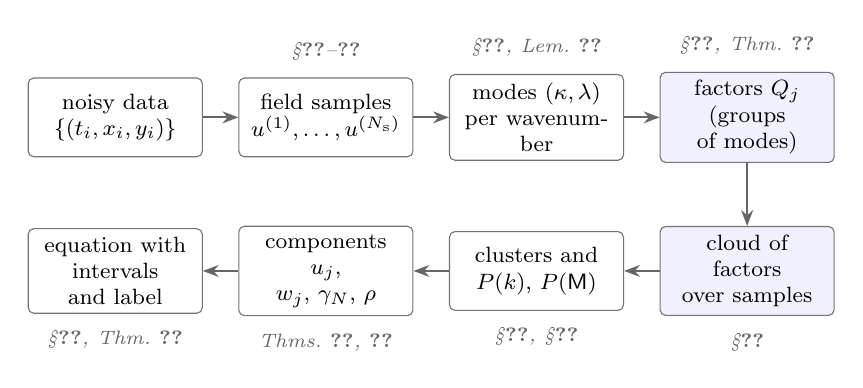
\begin{tikzpicture}[
  node distance=3.5mm and 4.5mm,
  box/.style={draw=black!55, rounded corners=2pt, align=center, font=\footnotesize, inner sep=3pt,
              minimum height=10mm, text width=20mm, fill=white},
  grp/.style={box, fill=blue!6},
  thy/.style={font=\scriptsize\itshape, text=black!60, align=center},
  arr/.style={-{Stealth[length=2mm]}, black!60, thick}]
\node[box] (data) {noisy data\\$\{(t_i,x_i,y_i)\}$};
\node[box, right=of data] (gp) {field samples\\$u^{(1)},\dots,u^{(\Nsamp)}$};
\node[box, right=of gp] (modes) {modes $(\kappa,\lambda)$\\per wavenumber};
\node[grp, right=of modes] (fac) {factors $Q_j$\\(groups of modes)};
\node[grp, below=8mm of fac] (cloud) {cloud of factors\\over samples};
\node[box, left=of cloud] (clus) {clusters and\\$P(k)$, $P(\Mfit)$};
\node[box, left=of clus] (split) {components $u_j$,\\$w_j$, $\gN$, $\rho$};
\node[box, left=of split] (out) {equation with\\intervals and label};
\draw[arr] (data)--(gp); \draw[arr] (gp)--(modes); \draw[arr] (modes)--(fac);
\draw[arr] (fac)--(cloud); \draw[arr] (cloud)--(clus); \draw[arr] (clus)--(split); \draw[arr] (split)--(out);
\node[thy, above=1mm of gp] {\S\ref{sec:alg-interp}--\ref{sec:nyquist}};
\node[thy, above=1mm of modes] {\S\ref{sec:alg-pencil}, Lem.~\ref{lem:ep}};
\node[thy, above=1mm of fac] {\S\ref{sec:alg-structfit}, Thm.~\ref{thm:factor}};
\node[thy, below=1mm of cloud] {\S\ref{sec:bayes-cloud}};
\node[thy, below=1mm of clus] {\S\ref{sec:alg-loop}, \S\ref{sec:bayes-cloud}};
\node[thy, below=1mm of split] {Thms.~\ref{thm:hm}, \ref{thm:eint}};
\node[thy, below=1mm of out] {\S\ref{sec:alg-labels}, Thm.~\ref{thm:ident}};
\end{tikzpicture}
\caption{The method at a glance. Shaded: the two grouping steps, of modes into factors within one sample and of
factors across samples. Each box names the section that describes it and the result that justifies it.}\label{fig:roadmap}
\end{figure}



\section{The analytical framework}\label{sec:analysis}
This section develops the grouping structure in the order in which the algorithm will use it: derivatives become
polynomials (\cref{sec:ring}); a solution carries an ideal of equations, and exponential-polynomials are exactly the
solutions that carry too little (\cref{sec:ann,sec:ep}); this decides when the equation can be recovered at all
(\cref{sec:ident,sec:certify}); the factors of the symbol split the solution, with projectors given by the eigenvalues
(\cref{sec:factor}); the split is stable exactly when the Friedrichs angle is positive (\cref{sec:cond}); and inside one
factor the additive terms interact (\cref{sec:eint}). \Cref{tab:notation} collects the notation.

% Shared module: notation table (one symbol, one meaning). Checked by tools/check_notation.py.
\begin{table}[htbp]
\centering\small
\caption{Notation for the analysis. Each symbol has one meaning throughout the paper; \cref{tab:notation-alg} lists the notation of the algorithm.}\label{tab:notation}
\begin{tabularx}{\linewidth}{@{}l X l@{}}
\toprule
Symbol & Meaning & Introduced\\
\midrule
\multicolumn{3}{@{}l}{\emph{Operators and their algebra}}\\
$\ring=\C[\tau,\xi]$ & ring of constant-coefficient operators; $\tau\leftrightarrow\partial_t$, $\xi\leftrightarrow\partial_x$ & \cref{def:ring}\\
$P,\ Q_j,\ P_i,\ e_i$ & an operator and its symbol; a factor; an irreducible factor and its multiplicity & \cref{sec:ring,sec:factor}\\
$\Var(P)$ & characteristic variety $\{P=0\}\subset\C^2$ & \cref{def:ring}\\
$\kappa,\ \lambda(\kappa)$ & real wavenumber ($\xi=i\kappa$); temporal rate of a mode & \cref{sec:ring}\\
$\Lambda_j(\xi)$ & branch of an evolution factor $Q_j=\tau-\Lambda_j(\xi)$ & \eqref{eq:lagrange}\\
$\Ann(u)$ & annihilator: all operators that kill $u$ & \cref{def:ann}\\
$\Gu,\ \Ju,\ \sigp(u)$ & intrinsic operator $\gcdop\Ann(u)$; cofactor ideal; point spectrum $\Var(\Ju)$ & \eqref{eq:GJ}\\
$\EP$ & exponential-polynomials & \cref{def:ep}\\
$N,\ \deltaP$ & number of factors; dimension of the overlap between their solution spaces & \cref{thm:factor}\\
$m_j,\ d_j$ & degree of factor $j$ in $\tau$ and in $\xi$ & \cref{sec:alg-loop}\\
\multicolumn{3}{@{}l}{\emph{Geometry and energy}}\\
$\sumop$ & sum operator $(u_1,\dots,u_N)\mapsto\sum_ju_j$ & \cref{sec:cond}\\
$\gN$ & conditioning constant of $\sumop$; error amplification $\gN^{-1/2}$ & \eqref{eq:gammaN}\\
$\cF,\ \thetaF$ & Friedrichs cosine and angle; $\gamma_2=1-\cF$ & \cref{sec:cond}\\
$\Hs$ & Sobolev space of index $s$ & \cref{sec:cond}\\
$K;\ \mathcal A_n,\ \flow_n,\ \Delta_n$ & number of additive terms of a factor; a term; its flow $e^{t\mathcal A_n}$; increment $\flow_n-\Id$ & \cref{sec:eint}\\
$\hat{\mathcal A}_n(\kappa)$ & Fourier symbol of the term $\mathcal A_n$ & \eqref{eq:eint-fourier}\\
$\Eint,\ \rho$ & interaction term; interaction ratio $\norm{\Eint}/\norm{u(T)-u_0}$ & \eqref{eq:eint-def}, \eqref{eq:energy}\\
$w_j$ & energy share of group $j$ & \eqref{eq:energy}\\
\bottomrule
\end{tabularx}
\end{table}

\begin{table}[htbp]
\centering\small
\caption{Notation for the algorithm (continued from \cref{tab:notation}).}\label{tab:notation-alg}
\begin{tabularx}{\linewidth}{@{}l X l@{}}
\toprule
Symbol & Meaning & Introduced\\
\midrule
$T,\ L$ & length of the time window; spatial period & \cref{sec:alg-interp}\\
$\Delta t,\ \Delta x;\ h$ & grid spacings; mean spacing $\sqrt{TL/n}$ of $n$ scattered points & \cref{sec:nyquist}\\
$\noise,\ \sigbin$ & observation noise standard deviation; its value in one Fourier bin & \cref{sec:alg-interp,sec:nyquist}\\
$\mathcal K,\ z$ & band of usable wavenumbers; detection threshold in units of $\sigbin$ & \cref{sec:nyquist}\\
$h_\kappa$ & spread $\max_{\ell,\ell'}\abs{\kappa_\ell-\kappa_{\ell'}}$ of the wavenumbers on which a factor is fitted & \cref{prop:counting}\\
$A_p,\ \sigma_{\lambda,p}$ & amplitude of mode $p$; standard deviation of its rate & \cref{sec:alg-pencil}\\
$\Nsamp,\ u^{(q)},\ \pi_q$ & number of posterior field samples; sample $q$; its weight & \cref{sec:alg-interp}\\
$\Mfit$ & a structure (number and degrees of the factors) & \cref{sec:alg-loop}\\
$B_j$ & orthonormal basis of the sampled kernel of $Q_j$ & \cref{sec:alg-interference}\\
$E_j$ & kernel exponentials of $Q_j$ evaluated at the observation points & \cref{sec:alg-accept}\\
$\omega^2$ & prior variance of the component coefficients & \eqref{eq:linmodel}\\
$\eta_r,\ \ell^{(r)}$ & amplitudes and length scales of the Gaussian-process kernel & \eqref{eq:gp}\\
$\eta,\ \eta_h,\ \pi_h,\ N_\eta$ & hyperparameters; a draw of them; its weight; number of draws & \eqref{eq:marginal-eta}\\
$\beta,\ \cloud$ & coefficient vector of a factor; cloud of factors & \eqref{eq:cloud}\\
$\alpha$ & concentration of the Dirichlet process & \cref{sec:bayes-cloud}\\
$k,\ \keff,\ \bar w_j$ & number of clusters (groups) found; effective number of groups; cluster masses & \cref{sec:bayes-cloud}\\
\FC, \IDK, \MIS, \UND & output labels & \cref{sec:alg-labels}\\
\bottomrule
\end{tabularx}
\end{table}

% Shared module: symbols, the operator ring, annihilators, the intrinsic operator.
\subsection{Derivatives become polynomials}\label{sec:ring}
Throughout, $\Omega\subset\R^2$ is a domain in the variables $(t,x)$ and every operator has constant
coefficients,
\[
  P(\partial_t,\partial_x)=\sum_{j,k}c_{jk}\,\partial_t^{\,j}\partial_x^{\,k},\qquad c_{jk}\in\C .
\]
The exponentials $\psi_{\tau,\xi}(t,x)=e^{\tau t+\xi x}$, $(\tau,\xi)\in\C^2$, are common eigenfunctions of
all such operators: $\partial_t \psi_{\tau,\xi}=\tau \psi_{\tau,\xi}$, $\partial_x \psi_{\tau,\xi}=\xi \psi_{\tau,\xi}$ and
therefore
\begin{equation}\label{eq:symbol-action}
  P(\partial)\,\psi_{\tau,\xi}=P(\tau,\xi)\,\psi_{\tau,\xi}.
\end{equation}
Differentiation is thus replaced by multiplication, and operators are replaced by polynomials.

\begin{definition}[Operator ring, symbol, characteristic variety]\label{def:ring}
The constant-coefficient operators form the commutative ring
$\ring=\C[\partial_t,\partial_x]\cong\C[\tau,\xi]$. The polynomial $P(\tau,\xi)$ is the \emph{symbol} of
$P(\partial)$, and its zero set $\Var(P)=\{(\tau,\xi)\in\C^2:P(\tau,\xi)=0\}$ is the
\emph{characteristic variety}.
\end{definition}

By \eqref{eq:symbol-action}, $\psi_{\tau,\xi}$ solves $P(\partial)u=0$ exactly when $(\tau,\xi)\in\Var(P)$.
A Fourier mode in space is the case $\xi=i\kappa$ with wavenumber $\kappa\in\R$; then
$P(\tau,i\kappa)=0$ is the \emph{dispersion relation}, and the roots $\tau=\lambda(\kappa)$ are the
temporal rates of the mode $e^{\lambda(\kappa)t+i\kappa x}$.

\paragraph{Convention}
We keep the algebraic variable $\xi$ in statements about the ring and write $\xi=i\kappa$ only when we
evaluate on Fourier modes. With this convention a symbol has real coefficients exactly when the
equation is real, and no factor $i$ ever appears inside $\ring$.

\begin{example}[Transport plus diffusion: the running example]\label{ex:tpd}
The operator $P=(\partial_t+c\,\partial_x)(\partial_t-\nu\,\partial_x^2)$, with speed $c>0$ and diffusivity
$\nu>0$, has symbol
\[
  P(\tau,\xi)=Q_1Q_2,\qquad Q_1=\tau+c\,\xi,\qquad Q_2=\tau-\nu\,\xi^2 .
\]
On Fourier modes the two factors give two dispersion branches, $\lambda_1(\kappa)=-ic\kappa$ (a
wave that travels without decay) and $\lambda_2(\kappa)=-\nu\kappa^2$ (a standing mode that decays).
A solution is any superposition of modes on the two branches. The equation is one object; its
\emph{two factors} are two groups of modes. Recovering those groups from data is the subject of this
paper. We use $c=1$, $\nu=0.3$ in all numerical illustrations.
\end{example}

\subsection{What a solution knows: the annihilator}\label{sec:ann}
A single function satisfies many equations: $e^{x}$ is annihilated by $\partial_x-1$, by
$\partial_x^2-1$ and by every multiple of $\partial_x-1$.

\begin{definition}[Annihilator]\label{def:ann}
For a distribution $u$ on $\Omega$, $\Ann(u)=\{Q\in\ring:\ Q(\partial)u=0\}$.
\end{definition}

$\Ann(u)$ is an ideal: it is closed under sums and under multiplication by any operator, because
$(SQ)(\partial)u=S(\partial)\big(Q(\partial)u\big)=0$. It collects every constant-coefficient equation
that $u$ satisfies. We use three classical facts about $\C[\tau,\xi]$~\cite{CLO15}:
unique factorization into irreducible polynomials; B\'ezout's theorem (two polynomials without a
common factor have finitely many common zeros); and Hilbert's Nullstellensatz (if $q$ vanishes on
the zero set $\Var(I)$ of an ideal $I$, then $q^k\in I$ for some $k$). All three require the complex
field, which is why symbols are always considered over $\C$.

\begin{lemma}[Splitting off the greatest common divisor]\label{lem:gcd}
Every nonzero ideal $I\subset\ring$ factors as $I=g\cdot J$, where $g=\gcdop(I)$ and $J$ is an ideal
with finite zero set $\Var(J)$.
\end{lemma}

The proof (\cref{app:proofs}) is elementary: divide by $g$, then use B\'ezout on two elements of $J$
without a common factor. Applied to $I=\Ann(u)$ the lemma gives the decomposition
\begin{equation}\label{eq:GJ}
  \Ann(u)=\Gu\,\Ju,\qquad \Gu=\gcdop\Ann(u),\qquad \sigp(u)=\Var(\Ju)\ \text{finite}.
\end{equation}
The polynomial $\Gu$ is the part of the equation that $u$ fills out along whole curves of $\C^2$;
the finite set $\sigp(u)$, the \emph{point spectrum} of $u$, lists the isolated exponentials that $u$
happens to contain. We call $\Gu$ the \emph{intrinsic operator} of $u$: it depends on $u$ alone,
whereas an annihilator $P$ supplied from outside may contain spurious factors.

\paragraph{Reading the two pieces}
The two objects in~\eqref{eq:GJ} answer different questions. The polynomial $\Gu$ is a differential
equation: its zero set $\Var(\Gu)$ is a union of curves in $\C^2$, and each curve is a continuous family of
exponential modes $e^{\tau t+\xi x}$, all solving $\Gu(\partial)v=0$. The point spectrum $\sigp(u)$ is a list: the
finitely many individual exponential modes that are present in this particular function $u$ and are not
accounted for by $\Gu$. In short, $\Gu$ identifies an equation that describes a whole family of modes;
$\sigp(u)$ identifies the isolated modes that $u$ happens to contain. \Cref{ex:extremes} shows the two
extreme cases.

\begin{example}[Two extremes]\label{ex:extremes}
For $u=e^{x}$, $\Ann(u)=(\tau,\ \xi-1)$ is the ideal of the single point $(0,1)$; hence $\Gu=1$ and
$\sigp(u)=\{(0,1)\}$: the function knows one exponential and no equation. For $u=f(x-ct)$ with a
profile $f$ that is not a finite sum of exponentials times polynomials,
$\Ann(u)=(\tau+c\xi)$; hence $\Gu=\tau+c\xi$ and $\sigp(u)=\emptyset$: the function knows its
equation completely (\cref{thm:ident}).
\end{example}

% Shared module: exponential-polynomials.
\subsection{Exponential-polynomials: the solutions that remember too little}\label{sec:ep}
\begin{definition}[Exponential-polynomials]\label{def:ep}
$\EP$ is the set of finite sums $\sum_{j}p_j(t,x)\,e^{\tau_jt+\xi_jx}$ with polynomials $p_j$ and
exponents $(\tau_j,\xi_j)\in\C^2$. $\EP(\Omega)$ denotes their restrictions to $\Omega$.
\end{definition}

For a function $w$ let $\ring w=\spn\{\partial_t^{\,j}\partial_x^{\,k}w:\ j,k\ge0\}$ be the space of all its
derivatives. The map $Q\mapsto Q(\partial)w$ is onto $\ring w$ with kernel $\Ann(w)$, so
$\ring w\cong\ring/\Ann(w)$ as vector spaces.

\begin{lemma}[Finite-dimension criterion]\label{lem:ep}
Let $\Omega$ be connected. Then $w\in\EP(\Omega)$ if and only if $\dim_\C\ring w<\infty$. In that case
$\Var(\Ann w)$ is the finite set of exponents $\{(\tau_j,\xi_j)\}$ that occur in $w$.
\end{lemma}

\begin{proof}[Proof idea]
We show that $w$ is an exponential-polynomial if and only if its derivatives span a finite-dimensional
space. ($\Rightarrow$) For one term $w=p(t,x)\,e^{at+bx}$,
\[
  \partial_tw=(p_t+a\,p)\,e^{at+bx},\qquad \partial_xw=(p_x+b\,p)\,e^{at+bx}.
\]
Differentiation never raises the degree of $p$, so every derivative of $w$ lies in the finite-dimensional space
of polynomials of degree at most $\deg p$ times $e^{at+bx}$; a finite sum of such terms stays in a finite sum of
such spaces. ($\Leftarrow$) If $\ring w$ is finite-dimensional, $\partial_t$ and $\partial_x$ map it to itself and act
on it as two commuting matrices $A$ and $B$. Their minimal polynomials $m_A$ and $m_B$ give two
constant-coefficient differential equations,
\[
  m_A(\partial_t)\,w=0,\qquad m_B(\partial_x)\,w=0,
\]
one in each variable. On every rectangle inside $\Omega$ their common solutions are exponential-polynomials, and
connectedness extends this representation to all of $\Omega$. The joint eigenvalues $(a,b)$ of $A$ and $B$ are
the exponents that occur in $w$. Details are in \cref{app:proofs}.
\end{proof}

\inbrief{Deciding whether $w\in\EP$ is a finite-dimensional linear-algebra question: compute the rank
of the derivatives of $w$. The joint eigenvalues of the two matrices are the exponents, that is, the
points of $\C^2$ at which $w$ lives. This is the computational core of everything that follows: the
matrix pencil of \cref{sec:alg-pencil} is exactly this eigenvalue computation, done for $\partial_t$
one wavenumber at a time.}

\begin{example}[Rich and poor solutions of the heat equation]\label{ex:heat-rich-poor}
A single heat mode $e^{-\nu\kappa^2t+i\kappa x}$ and any finite sum of such modes belong to $\EP$.
The heat kernel $t^{-1/2}e^{-x^2/(4\nu t)}$ does not: its $x$-derivatives are polynomials of
increasing degree times the same Gaussian, so they span an infinite-dimensional space.
\end{example}

% Shared module: identification, uniqueness, the spectral form, limits of certification.
\subsection{When does a solution determine its equation?}\label{sec:ident}
Let $\Omega$ be open and connected (on a disconnected set the pieces may obey different equations),
let $u\in\mathcal D'(\Omega)$ satisfy $P(\partial)u=0$, and let $P=\prod_iP_i^{e_i}$ (up to a nonzero constant factor) be the
factorization of $P$ into pairwise non-associate irreducible polynomials $P_i$ with multiplicities
$e_i$. The question is whether $\Ann(u)=(P)$: then every constant-coefficient equation satisfied by
$u$ is a consequence of $P$, and $P$ is determined by $u$.

\begin{theorem}[Identification criterion]\label{thm:ident}
Put $v_i=(P/P_i)(\partial)\,u$ and $v_i'=(P/P_i^{e_i})(\partial)\,u$.
\begin{enumerate}[label=(\alph*)]
  \item $\Ann(u)=(P)$ if and only if $v_i\notin\EP(\Omega)$ for every $i$.
  \item $\Var(\Ann u)=\Var(P)$ if and only if $v_i'\notin\EP(\Omega)$ for every $i$.
  \item If $P$ is square-free, (a) and (b) coincide. If $P$ is monic in $\tau$ of degree $m$, then
  $\Ann(u)=(P)$ if and only if the only $(\varphi_0,\dots,\varphi_{m-1})\in\C[\xi]^m$ with
  $\sum_{j<m}\varphi_j(\partial_x)\,\partial_t^{\,j}u=0$ is zero.
\end{enumerate}
\end{theorem}

The idea is to strip one irreducible factor and look at what is left. The function $v_i$ solves
$P_i(\partial)v_i=0$. If $v_i$ is a generic solution of that factor, no smaller operator kills $u$.
If $v_i$ is an exponential-polynomial, some $h$ coprime to $P_i$ kills it, and then
$h\cdot P/P_i$ is an annihilator of $u$ that is not a multiple of $P$. The converse uses
\cref{lem:gcd}; the full proof is in \cref{app:proofs}.

\begin{proposition}[Uniqueness and the intrinsic operator]\label{prop:unique}
\begin{enumerate}[label=(\alph*)]
  \item If $\Ann(u)=(P)$, then $P$ is determined by $u$ up to a nonzero constant and is the unique
  annihilator of minimal degree.
  \item $\Ann(u)=(P)$ if and only if $\sigp(u)=\emptyset$ and $\Gu\sim P$ (equality up to a constant).
  \item For any annihilator $P$, the multiplicity of $P_i$ in $\Gu$ equals $e_i-\max\{k\le e_i:
  (P/P_i^{k})(\partial)u\in\EP\}$. Hence $\Gu$ is computed from any annihilator by at most
  $\sum_ie_i$ membership tests ``$\in\EP$''.
\end{enumerate}
\end{proposition}

\begin{example}[The heat equation, continued]\label{ex:heat-ident}
For $P=\tau-\nu\xi^2$ (irreducible) the criterion reads: $\Ann(u)=(P)$ if and only if $u\notin\EP$.
One mode $e^{-\nu\kappa^2t+i\kappa x}$ has $\Ann(u)=(\tau+\nu\kappa^2,\ \xi-i\kappa)$, a point of
$\Var(P)$; it cannot distinguish the heat equation from the pure decay $\partial_t+\nu\kappa^2$, or from
any other equation whose variety passes through the point $(-\nu\kappa^2,i\kappa)$. The heat kernel is not in $\EP$, so every
constant-coefficient equation it satisfies is a multiple of $\partial_t-\nu\partial_x^2$.
\end{example}

\begin{remark}[Curves and points]\label{rem:curves-points}
The two cases of \cref{ex:heat-ident} sit at the two ends of the decomposition~\eqref{eq:GJ}. A finite sum of modes
$u\in\EP$ has an annihilator with finitely many zeros, so
\[
  u\in\EP:\qquad \Gu=1,\qquad \sigp(u)=\{(\tau_j,\xi_j)\}\ \text{finite (its exponents)},
\]
whereas the zero set of a nonconstant polynomial in two variables is a whole algebraic curve. For the heat kernel
the situation is reversed:
\[
  u=t^{-1/2}e^{-x^2/(4\nu t)}:\qquad \Gu=\tau-\nu\xi^2,\quad \Var(\Gu)\ \text{a curve},\qquad \sigp(u)=\emptyset .
\]
By \cref{prop:unique}(b) it is exactly this pair, an empty point spectrum together with $\Gu\sim P$, that gives
$\Ann(u)=(P)$: the solution fills the whole curve of its equation and contains no isolated mode besides.
\end{remark}

\roleinalg{Data never contain the heat kernel, they contain finitely many sampled modes; a finite
set of modes is always an exponential-polynomial. The algorithm therefore never claims that an
equation is \emph{identified}. It asks whether the modes it sees are \emph{compatible} with a factored
symbol and are rich enough in each factor (enough distinct wavenumbers per branch) for the factor to
be pinned down within its class. This is the meaning of the label \FC{} in \cref{sec:alg-labels}.}

\subsection{What finite data can and cannot certify}\label{sec:certify}
\Cref{thm:ident} speaks about $u$, not about finitely many numbers. Two facts frame what an algorithm
can promise.

Recall that $\ring u=\spn\{\partial_t^{\,j}\partial_x^{\,k}u:\ j,k\ge0\}$ is the vector space generated by the
derivatives of $u$ (\cref{sec:ep}). The \emph{jet} of order $M$ of $u$ at a point $z_0=(t_0,x_0)$ is the list of its
derivatives of order at most $M$ at that point; for example
\[
  j^2_{z_0}(u)=\big(u,\ u_t,\ u_x,\ u_{tt},\ u_{tx},\ u_{xx}\big)\big|_{(t,x)=z_0}.
\]

\begin{proposition}[Finite data]\label{prop:certify}
Let $\Omega$ be connected and $z_0\in\Omega$.
\begin{enumerate}[label=(\roman*)]
  \item If $\dim_\C\ring u\le n$, the jet of order $2n-1$ of $u$ at $z_0$ determines $\Ann(u)$ among all functions
  $u'$ with $\dim_\C\ring u'\le n$.
  \item For every $u$ and every $M$ there is a polynomial, hence an exponential-polynomial, with the same jet of
  order $M$ at $z_0$; and for finitely many sample points there is an exponential-polynomial with the same values.
  Consequently, without a bound on $\dim\ring u$, no finite set of jets or samples proves $\Ann(u)=(P)$.
\end{enumerate}
\end{proposition}

\begin{proof}
(ii) The Taylor polynomial of order $M$ at $z_0$ has the same jet, and polynomial interpolation in two variables
matches any finite set of values. Both are exponential-polynomials, and an exponential-polynomial never has
$\Ann=(P)$ when $P$ has an irreducible factor (\cref{thm:ident}: all $v_i$ are then exponential-polynomials).
(i) The space $\ring u$ is invariant under differentiation and, by \cref{lem:ep}, consists of real-analytic
exponential-polynomials. Let $K_M$ be the subspace of elements of $\ring u$ whose jet of order $M$ vanishes at $z_0$.
Then $K_{M+1}=\{f\in K_0:\ \partial_tf,\partial_xf\in K_M\}$, so once $K_{M+1}=K_M$ the chain is constant, and a
constant $K_M$ is a derivative-invariant space of functions vanishing at $z_0$ with all their derivatives, hence
$\{0\}$. Since $\dim K_0\le n-1$, the chain reaches $\{0\}$ by $M=n-1$: the jet of order $n-1$ at $z_0$ is injective
on $\ring u$, and likewise on $\ring u'$. For $Q$ of degree at most $n$, $Q\in\Ann(u)$ iff the jet of order
$n-1$ of $Q(\partial)u$ vanishes at $z_0$, a condition on the jet of order $2n-1$ of $u$; the same holds for $u'$.
Finally $\Ann(u)$ has codimension at most $n$, so a Gr\"obner basis for a degree-compatible order consists of
polynomials of degree at most $n$; the same holds for $\Ann(u')$, and two ideals generated in degree at most $n$
that contain the same polynomials of degree at most $n$ are equal.
\end{proof}

The consequence for learning is a design rule: without an a priori bound on $\dim\ring u$, which data never
supply, an algorithm can refute a candidate equation, or report that it is compatible with the data at
the resolution available, but it cannot certify it. Its output must carry a label that says which of these
happened.

% Shared module: the grouping theorem (factor decomposition), projectors, why terms fail, holes.
\subsection{Groups are factors, not terms}\label{sec:factor}
Suppose the operator is known and factored as
\begin{equation}\label{eq:factored}
  P=P_1^{e_1}\cdots P_N^{e_N},\qquad Q_j=P_j^{e_j}\ \text{pairwise coprime}.
\end{equation}
Two ways of splitting a solution suggest themselves: one piece per \emph{factor} $Q_j$, or one piece
per additive \emph{term} of the operator (for $u_t=\nu u_{xx}-cu_x$, one piece for diffusion and one
for transport). Only the first works.

\begin{theorem}[Factor decomposition]\label{thm:factor}
Let $\Omega\subset\R^2$ be bounded, connected and simply connected, and let $P$ be as in
\eqref{eq:factored}. Every $u\in\ker P(\partial)$ (in $\mathcal D'(\Omega)$ or $C^\infty(\Omega)$) can be
written
\begin{equation}\label{eq:decomp}
  u=\sum_{j=1}^N u_j,\qquad Q_j(\partial)\,u_j=0 .
\end{equation}
The tuples $(u_1,\dots,u_N)$ that sum to zero form a space of exponential-polynomials of dimension
exactly
\begin{equation}\label{eq:deltaP}
  \deltaP=\sum_{i<j}\dim_\C\ring/(Q_i,Q_j),
\end{equation}
the number of intersection points of the varieties $\Var(Q_i)$, counted pair by pair and with multiplicity.
\end{theorem}

The number $\dim_\C\ring/(Q_i,Q_j)$ therefore has two readings at once. Geometrically it counts the points where
the curves $\Var(Q_i)$ and $\Var(Q_j)$ meet, with multiplicity. Analytically it is the dimension of the space of
exponential-polynomials that solve both $Q_i$ and $Q_j$, one exponential for each meeting point (times polynomials at a
point of higher multiplicity). For two groups these are exactly the functions that can be moved from one group to the
other without changing $u$: each meeting point of the two curves is one shared mode. For three or more groups $\deltaP$
still gives the dimension of the ambiguity, but the ambiguous tuples need not be sums of modes shared by pairs.

In one variable the statement is B\'ezout's identity: if $aQ_1+bQ_2=1$, then
$u=bQ_2u+aQ_1u$ splits $u$ into a solution of $Q_1$ and a solution of $Q_2$. In two variables
``coprime'' no longer gives $1\in(Q_1,Q_2)$; it only gives finitely many common zeros, and the
finite-dimensional quotient $\ring/(Q_1,Q_2)$ measures exactly how much the two groups overlap. The
proof combines the exact sequence
$0\to\ring/(Q_1Q_2)\to\ring/(Q_1)\oplus\ring/(Q_2)\to\ring/(Q_1,Q_2)\to0$ with the vanishing of the obstruction
$\operatorname{Ext}^1(M,C^\infty(\Omega))$ for the finite-dimensional module $M=\ring/(Q_1,Q_2)$, which reduces to
$H^1_{dR}(\Omega)=0$ (compare the fundamental principle of Ehrenpreis and Palamodov~\cite{Ehr70,Pal70});
see \cref{app:proofs}.

\begin{example}[Running example: two groups with a two-dimensional overlap]\label{ex:tpd-factor}
For $Q_1=\tau+c\xi$ and $Q_2=\tau-\nu\xi^2$ the common zeros are $(0,0)$ and $(c^2/\nu,-c/\nu)$,
both simple, so $\deltaP=2$. The ambiguity is spanned by the constant function and by
$e^{(c^2/\nu)t-(c/\nu)x}$: a constant (or that growing exponential) can be moved from one group to
the other without changing $u$. Among Fourier modes ($\xi=i\kappa$, $\kappa\in\R$) only the
first point is visible: the $\kappa=0$ mode belongs to both groups.
\end{example}

\paragraph{Projectors from the eigenvalues}
When each factor is an evolution factor, $Q_j=\tau-\Lambda_j(\xi)$ with pairwise distinct branches
$\Lambda_j$, a component is an eigenfunction of $\partial_t$: $\partial_tu_j=\Lambda_j(\partial_x)u_j$. Applying
$\prod_{k\ne j}(\partial_t-\Lambda_k(\partial_x))$ to $u=\sum_lu_l$ removes every $u_l$ with $l\ne j$ and multiplies $u_j$ by $\prod_{k\ne j}(\Lambda_j-\Lambda_k)(\partial_x)$.
On a spatial Fourier mode $\kappa$ at which no two branches meet this factor is a nonzero number, hence
\begin{equation}\label{eq:lagrange}
  \hat u_j=\prod_{k\ne j}\frac{\partial_t-\Lambda_k(i\kappa)}{\Lambda_j(i\kappa)-\Lambda_k(i\kappa)}\;\hat u(t,\kappa) .
\end{equation}
This is a multiplier, rational in $\kappa$, with poles exactly where two branches
meet ($\Lambda_j(i\kappa)=\Lambda_k(i\kappa)$), that is, at the visible part of the overlap counted by $\deltaP$.
Formula~\eqref{eq:lagrange} is the Lagrange interpolation formula for the spectral projectors of a
matrix with distinct eigenvalues, applied to $\partial_t$ restricted to one wavenumber: the
\emph{eigenvalues decide the groups}. For the running example,
$\hat u_1(t,\kappa)=\big(\partial_t+\nu\kappa^2\big)\hat u/\big(\nu\kappa^2-ic\kappa\big)$, which is
singular only at $\kappa=0$.

\paragraph{Why additive terms do not form groups}
\begin{proposition}[Terms do not give components]\label{prop:terms}
If $P=\mathcal A_1+\mathcal A_2$ with constant coefficients, then
$\ker P\cap(\ker \mathcal A_1+\ker \mathcal A_2)\subseteq\ker P\cap\ker(\mathcal A_1\mathcal A_2)$, and the right-hand side is
finite-dimensional whenever $\Var(\mathcal A_1)\cap\Var(\mathcal A_2)$ is finite.
\end{proposition}

\begin{proof}
If $u=a+b$ with $\mathcal A_1a=0$ and $\mathcal A_2b=0$, then $\mathcal A_1\mathcal A_2u=\mathcal A_2\mathcal A_1a+\mathcal A_1\mathcal A_2b=0$ because the operators commute.
At a common zero of $P$ and $\mathcal A_1\mathcal A_2$ either $\mathcal A_1=0$, and then $\mathcal A_2=P-\mathcal A_1=0$, or $\mathcal A_2=0$ and then
$\mathcal A_1=0$; so $\Var(P,\mathcal A_1\mathcal A_2)=\Var(\mathcal A_1)\cap\Var(\mathcal A_2)$. When this set is finite, the ideal $(P,\mathcal A_1\mathcal A_2)$
has finite codimension, its common kernel consists of exponential-polynomials with exponents in that
set (\cref{lem:ep}), and it is finite-dimensional.
\end{proof}

For the heat equation, $\mathcal A_1=\partial_t$ and $\mathcal A_2=-\nu\partial_x^2$: every sum $f(x)+a(t)+b(t)x$ of a
solution of $\mathcal A_1$ and one of $\mathcal A_2$ is killed by $\mathcal A_1\mathcal A_2\sim\partial_t\partial_x^2$, while a heat mode
$e^{-\nu\kappa^2t}\cos\kappa x$ is not. A generic heat solution is \emph{not} ``a diffusion part plus a
stationary part''. The leftover of any term-wise split is the interaction term of
\cref{sec:eint}.

\paragraph{Where the decomposition fails}
The hypotheses of \cref{thm:factor} are not technical. On a disconnected domain different pieces
can satisfy different equations. On a domain with a hole the decomposition can fail: the Laplacian
factors as $(\partial_x+i\partial_y)(\partial_x-i\partial_y)$, yet $\log\abs{z}^2$ is harmonic on an annulus
and is not a sum of a holomorphic and an antiholomorphic single-valued function. The obstruction is
the first de Rham cohomology of $\Omega$, which is why the algorithm works on rectangles.

\roleinalg{\Cref{thm:factor} is the grouping principle of the paper. The objects that a learning
algorithm should group are \emph{modes of the same factor}; equivalently, points of the data's
Fourier--Laplace spectrum lying on the same irreducible component of $\Var(P)$. The overlap $\deltaP$
is the irreducible amount of ambiguity, and the algorithm resolves it by a fixed convention
(\cref{sec:alg-components}).}

% Shared module: conditioning of the split, Friedrichs angle, regularity.
\subsection{How well separated are the groups? The Friedrichs angle}\label{sec:cond}
\Cref{thm:factor} is algebraic: it says that the split exists, not that it is stable. Stability is a
geometric property of the component spaces $M_j=\ker_{\Hs}Q_j$, the solutions of each factor in the
Sobolev space $\Hs(\Omega)$. Let
\[
  \sumop:\ \textstyle\bigoplus_{j=1}^N M_j\to\Hs(\Omega),\qquad \sumop(u_1,\dots,u_N)=\sum_ju_j,
\]
be the \emph{sum operator}, with $\norm{(u_1,\dots,u_N)}^2=\sum_j\norm{u_j}_{\Hs}^2$, and define the
\emph{conditioning constant}
\begin{equation}\label{eq:gammaN}
  \gN=\inf_{0\ne v\perp\ker\sumop}\frac{\norm{\sumop v}^2}{\norm{v}^2}
  =\inf\sigma\big(\sumop^*\sumop\big|_{(\ker\sumop)^\perp}\big).
\end{equation}
It is the worst case, over all tuples of pieces, of the size of the sum relative to the size of the
pieces. Tuples in $\ker\sumop$ (the overlap of \cref{thm:factor}) are excluded. By the triangle and Cauchy--Schwarz inequalities,
$\norm{\sum_ju_j}^2\le\big(\sum_j\norm{u_j}\big)^2\le N\sum_j\norm{u_j}^2$, hence
\[
  0\le\gN\le N .
\]
If the spaces are mutually orthogonal, $\norm{\sum_ju_j}^2=\sum_j\norm{u_j}^2$ and $\gN=1$. At the other end, if $M_2$
approaches $M_1$ one can take $u_2\approx-u_1$: the pieces stay of unit size while their sum becomes arbitrarily
small, so $\gN\to0$. A small $\gN$ is the signature of groups that can almost cancel each other.

For two groups, $\gamma_2=1-\cF$, where the \emph{Friedrichs cosine}
\[
  \cF=\sup\big\{\abs{\ip ab}:\ a\in M_1\ominus(M_1\cap M_2),\ b\in M_2\ominus(M_1\cap M_2),\
  \norm a=\norm b=1\big\}=\cos\thetaF
\]
is the cosine of the smallest nonzero angle $\thetaF$ between the two spaces
(\cref{fig:friedrichs})~\cite{Deu01}. In regression terms, $M_1$ and $M_2$ are two blocks of regressors and $\cF$ is the
largest correlation between a combination of the first block and one of the second: the closer the blocks are to
collinear, the less the data can attribute to each.

\begin{theorem}[Stability of the split]\label{thm:hm}
Every $u\in\ker_{\Hs}P$ has components $u_j\in\Hs$ if and only if $\sum_jM_j$ is closed and dense in
$\ker_{\Hs}P$. Closedness is equivalent to $\gN>0$, and then
\begin{equation}\label{eq:stability}
  \Big(\sum_j\norm{u_j}_{\Hs}^2\Big)^{1/2}\le\gN^{-1/2}\,\norm{u}_{\Hs}
\end{equation}
for the minimum-norm components. If the component spaces are finite-dimensional, as for the sampled
kernels used by the algorithm, the sum is always closed and density holds whenever the sampled kernel of
$P$ is spanned by those of its factors, so stability reduces to $\gN>0$.
\end{theorem}

Density in $\Hs$ is a genuine condition on infinite-dimensional spaces. On convex domains solutions of
$P(\partial)u=0$ are limits of exponential solutions, uniformly on compact subsets~\cite{Mal56,Hor90},
and every exponential solution lies in $\sum_jM_j$; whether this extends to the $\Hs$ norm up to the boundary
for general $P$ we do not claim.

Two warnings come with the theorem. First, $\gN>0$ can fail on infinite-dimensional component spaces: the pieces of a smooth $u$ may then be
one derivative rougher than $u$ itself. Second, for $N\ge3$ groups the pairwise cosines do not
determine $\gN$: two pairs can be well separated while the three spaces are nearly dependent, so the
full Gram operator of $\sumop$ must be used.

\begin{figure}[tbp]
\centering
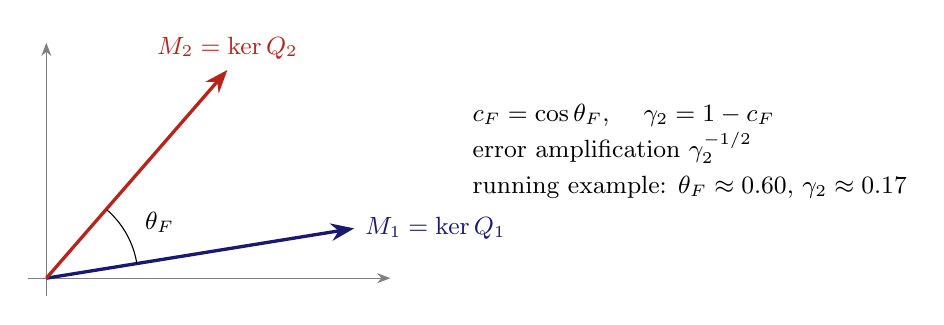
\begin{tikzpicture}[scale=1.15,>=Stealth]
  \draw[->,gray] (-0.2,0)--(3.8,0); \draw[->,gray] (0,-0.2)--(0,2.6);
  \draw[very thick,->,color=MidnightBlue] (0,0)--(3.4,0.55) node[right]{\small $M_1=\ker Q_1$};
  \draw[very thick,->,color=BrickRed] (0,0)--(2.0,2.3) node[above]{\small $M_2=\ker Q_2$};
  \draw (1.0,0.16) arc (9.2:49:1.0); \node at (1.25,0.62) {\small$\thetaF$};
  \node[anchor=west,align=left,font=\small] at (4.6,1.4)
   {$\cF=\cos\thetaF$, \quad $\gamma_2=1-\cF$\\[2pt]
    error amplification $\gamma_2^{-1/2}$\\[2pt]
    running example: $\thetaF\approx0.60$, $\gamma_2\approx0.17$};
\end{tikzpicture}
\caption{The Friedrichs angle $\thetaF$ between the solution spaces of two factors. A small angle
means that large pieces can almost cancel, so recovering the pieces from their sum amplifies errors by
up to $\gamma_2^{-1/2}=(1-\cos\thetaF)^{-1/2}$. The values quoted are those measured on the running
example in \cref{sec:worked}.}\label{fig:friedrichs}
\end{figure}

\roleinalg{$\gN$ is computed on the sampled kernel bases and reported with every result.
It enters twice: as the error amplification $\gN^{-1/2}$ of the components, and through the Bayesian
split layer (\cref{sec:bayes-split}), whose credible intervals widen and whose split probability
returns to the prior as $\thetaF\to0$. A small angle is therefore never hidden: it shows up as wide
intervals, not as a confident but wrong split.}

% Shared module: interaction term and energy.
\subsection{Inside one group: the interaction term and its energy}\label{sec:eint}
A single factor may have several additive terms: $Q_2=\tau-\nu\xi^2$ has one, but the advection--diffusion
factor $\tau+c\xi-\nu\xi^2$ has two. \Cref{prop:terms} says that such a factor cannot be split further
into one solution per term. We now measure exactly what is left over.

Consider an evolution $u_t=\mathcal Au$ with $\mathcal A=\mathcal A_1+\dots+\mathcal A_K$ (the terms), the flow $\flow(t)=e^{t\mathcal A}$ and the
flows of the single terms $\flow_n(t)=e^{t\mathcal A_n}$. If term $n$ acted alone it would change the datum by
$\Delta_nu_0=(\flow_n(t)-\Id)u_0$. The \emph{interaction term} is the part of the evolution that is not
the sum of these single-term changes,
\begin{equation}\label{eq:eint-def}
  \Eint(t)=u(t)-u_0-\sum_{n=1}^K\big(\flow_n(t)u_0-u_0\big).
\end{equation}

\begin{theorem}[Interaction term]\label{thm:eint}
If the terms commute (in particular, for constant coefficients),
\[
  \Eint(t)=\Big[\prod_{n=1}^K(\Id+\Delta_n)-\Id-\sum_{n=1}^K\Delta_n\Big]u_0
  =\sum_{\mathcal E\subseteq\{1,\dots,K\},\ \abs{\mathcal E}\ge2}\Big(\prod_{n\in\mathcal E}\Delta_n\Big)u_0 .
\]
For two terms $\Eint=\Delta_1\Delta_2u_0$. On Fourier modes, with symbols $\hat{\mathcal A}_n(\kappa)$ of the terms,
\begin{equation}\label{eq:eint-fourier}
  \widehat{\Eint}(t,\kappa)=\Big[\prod_ne^{t\hat{\mathcal A}_n(\kappa)}-1-\sum_n\big(e^{t\hat{\mathcal A}_n(\kappa)}-1\big)\Big]\hat u_0(\kappa).
\end{equation}
\end{theorem}

\begin{proof}
Commuting terms give $\flow=\prod_n\flow_n=\prod_n(\Id+\Delta_n)$. Expanding the product over subsets
$\mathcal E\subseteq\{1,\dots,K\}$ and removing the subsets with zero or one element gives the formula; on
Fourier modes every operator is multiplication by a number.
\end{proof}

Formula~\eqref{eq:eint-fourier} costs $O(K)$ operations per wavenumber, although writing out all
cross terms would need $2^K-K-1$ of them. For advection--diffusion,
$\abs{\widehat{\Eint}}/\abs{\hat u_0}=\abs{(e^{-ic\kappa t}-1)(e^{-\nu\kappa^2t}-1)}\le2$: the interaction
is of the same size as the solution, so it is not a small correction that a regularizer could remove.

\begin{proposition}[No stable removal]\label{prop:discont}
Let $Q=\tau+c\xi-\nu\xi^2$ (advection--diffusion, terms $-c\partial_x$ and $\nu\partial_x^2$) on a bounded
rectangle $\Omega=(0,T)\times(a,b)$. For every $s\ge0$,
\[
  \sup\Big\{\norm{\Eint}_{L^2(\Omega)}/\norm{u}_{\Hs(\Omega)}:\ u\in\EP,\ Q(\partial)u=0,\ u\ne0\Big\}=\infty,
\]
so $u\mapsto\Eint$ has no continuous extension to $\ker_{\Hs}Q$. Moreover, a solution of $Q(\partial)u=0$ is a
sum $v+w$ of solutions of the single-term evolutions $(\partial_t+c\partial_x)v=0$ and $(\partial_t-\nu\partial_x^2)w=0$ only
if it lies in a finite-dimensional space of exponential-polynomials.
\end{proposition}

The test solutions are $e^{\lambda_\zeta t+\zeta x}$ with real $\zeta>c/\nu$ and $\lambda_\zeta=\nu\zeta^2-c\zeta$, legitimate
data on a bounded interval: diffusion alone amplifies them by $e^{\nu\zeta^2t}$, the solution grows only like
$e^{\lambda_\zeta t}$, and the interaction must cancel a difference that grows faster than any power of $\zeta$
(\cref{app:proofs}). On a periodic domain with bounded wavenumbers the Fourier multiplier above is bounded by
$2$; the instability comes from the non-periodic window, which is the situation of real data. The second
statement means that a model which writes the data as a sum of single-term pieces, with any penalty on the
pieces, leaves a remainder on generic data, and that remainder is the interaction.

\paragraph{Energy}
We measure the size of a group and of the interaction by $L^2$ energies on the observation window.
The \emph{energy share} of group $j$ and the \emph{interaction ratio} are
\begin{equation}\label{eq:energy}
  w_j=\frac{\norm{u_j}}{\sum_k\norm{u_k}},\qquad
  \rho=\frac{\norm{\Eint(T)}}{\norm{u(T)-u_0}} ,
\end{equation}
where $T$ is the length of the time window. The shares $w_j$ say how much of the data each group
explains; $\rho$ says how far the evolution inside a multi-term factor is from the superposition of its
terms ($\rho=0$ for a factor with a single term). Interactions occur only \emph{inside} a factor:
different factors superpose exactly, which is another way of saying that factors, not terms, are the
right groups.

\roleinalg{By \cref{prop:discont}, a value of $\Eint$ computed from one interpolated field on a
bounded window is not reliable. The algorithm reports the distribution of $\rho$ over posterior samples
(\cref{sec:bayes-cloud}), never a single number, and uses the shares $w_j$ with credible intervals.}


\section{Nonlinear equations: why grouping gets harder}\label{sec:nonlinear}
This section is an outlook: it explains which parts of the grouping structure are lost for nonlinear equations and
which survive, and a reader interested in the method can go directly to \cref{sec:algorithm}. The one fact used later
is that the interaction term, unlike the groups, is still defined.

% Shared module: what changes for nonlinear equations (short, clearly an outlook).
The results above rest on one structure: candidate equations form the commutative ring
$\ring=\C[\tau,\xi]$, solutions form vector spaces, and the exact sequence behind \cref{thm:factor} (a Chinese
remainder theorem up to the finite overlap $\deltaP$) turns a
factorization of the symbol into a splitting of the solution. For a nonlinear equation
$u_t=\sum_n\mathcal A_n(u)$, with each $\mathcal A_n$ a polynomial in the jet $(u,u_x,u_{xx},\dots)$, this structure is lost
in three ways.
\begin{enumerate}[label=(\roman*)]
  \item \emph{No ring of candidates.} Products of nonlinear operators are not operators of the same kind
  in any useful sense, and there is no unique factorization. One fixes instead a finite
  \emph{dictionary} $\mathcal D$ of jet monomials of bounded degree and order, with span $\mathcal V$, and asks
  which relations $F(u,u_x,\dots)=0$ in $\mathcal V$ the data satisfy. In practice each monomial (for instance
  $u_t$, $u_x$, $u_{xx}$, $uu_x$, $u^2$) is evaluated at the sample points, giving a matrix $\Theta$ with one column per
  monomial; a relation $F=\sum_mc_m\,m(u)$ is a vector $c$ with $\Theta c\approx0$, so the candidate equations are the
  near-null space of $\Theta$.
  \item \emph{No superposition.} Solutions do not form a vector space, so ``the component of $u$ along a
  factor'' has no meaning; the groups of \cref{thm:factor} do not exist.
  \item \emph{Identification is relative.} Identification can only hold relative to $\mathcal V$ and modulo the
  differential consequences of $F$ (its derivatives $\partial_xF,\partial_x^2F,\dots$ are also relations in
  any rich dictionary). The precise statement is an exact sequence relating the relations of $u$ in $\mathcal V$
  to those generated by $F$; identification holds exactly when a jet-level obstruction vanishes.
\end{enumerate}

What survives is the interaction term. Definition~\eqref{eq:eint-def} still makes sense with the
nonlinear single-term flows, and its short-time expansion is
\begin{equation}\label{eq:jet}
  \Eint(t)=\frac{t^2}{2}\sum_{n\ne m}\mathcal A_n'[u_0]\big(\mathcal A_m(u_0)\big)+O(t^3),
\end{equation}
where $\mathcal A_n'[u_0]$ is the Fr\'echet derivative of $\mathcal A_n$ at $u_0$. For Burgers' equation
$u_t=-uu_x+\nu u_{xx}$ the two terms are $\mathcal A_1(u)=-uu_x$ and $\mathcal A_2(u)=\nu u_{xx}$, with Fr\'echet
derivatives $\mathcal A_1'[u](v)=-(vu_x+uv_x)$ and $\mathcal A_2'[u](v)=\nu v_{xx}$. Then
\[
  \mathcal A_1'[u_0]\big(\mathcal A_2(u_0)\big)=-\nu\,(u_0''u_0'+u_0u_0'''),\qquad
  \mathcal A_2'[u_0]\big(\mathcal A_1(u_0)\big)=-\nu\,(3u_0'u_0''+u_0u_0'''),
\]
and half their sum gives
\[
  \Eint(t)=-\nu\,\big(u_0u_0'''+2u_0'u_0''\big)\,t^2+O(t^3).
\]
The expansion holds only while the solution is smooth. The flow of the single term $-uu_x$ is the inviscid
Burgers equation, whose characteristics cross: for $u_0=\sin x$ they are $x=\xi+t\sin\xi$, and
$\partial x/\partial\xi=1+t\cos\xi$ first vanishes at $\xi=\pi$, $t^*=1$. After this breaking time the single-term flow
has a jump, $\Eint$ has a jump in $x$ whose height does not vanish as $\nu\to0$, and the interaction can only be measured in
$L^1$, where for a single shock it is small, of order $\nu$ up to logarithmic factors (a rate we do not prove here).
Whether such data still identify the equation relative to a dictionary depends on how many shocks they contain
compared with the degree of the dictionary; we do not pursue this here.

\paragraph{Variable coefficients}
If the coefficients depend on $(t,x)$, the operators form the Weyl algebra $\C[t,x]\langle\partial_t,\partial_x\rangle$, which
is not commutative ($\partial_x\,x-x\,\partial_x=1$). Annihilators become left ideals, factorizations are no longer unique,
and \cref{thm:factor} has no general analogue. Worse, if the coefficients may be arbitrary smooth functions, one solution
identifies nothing: any $u$ without zeros satisfies the first-order equation $\big(\partial_x-u_x/u\big)u=0$, whose
coefficient is built from $u$ itself. Identification becomes possible only inside a fixed, finite-dimensional class of
coefficients. For the Schr\"odinger equation $iu_t=-u_{xx}+V(x)u$, for instance, the potential is read off directly as
$V(x)=(iu_t+u_{xx})/u$ wherever $u\neq0$. In the spectral picture of \cref{sec:alg-pencil}, slowly varying coefficients
would make the rates depend on position, $\lambda(\kappa;x)$ (\cref{rem:varcoef}).

\paragraph{A possible route} The grouping idea can be carried over by replacing ``modes on the same
irreducible component of $\Var(P)$'' with ``jet samples satisfying the same relation in $\mathcal V$''. Locally
in time, \eqref{eq:jet} shows that a nonlinear flow is a linear one (its Fr\'echet derivative) plus a
quadratic correction, so one can group linearized modes on short windows and test, through the size
of $\Eint$, whether the groups persist. We do not pursue this here: without a ring there is no
analogue of $\deltaP$, of the projectors~\eqref{eq:lagrange} or of $\gN$, and these are what make the
linear algorithm verifiable.

\begin{table}[tbp]
\centering\small
\caption{What carries over beyond scalar linear equations with constant coefficients. ``Groups'' means a splitting of
a solution into pieces attached to pieces of the equation.}\label{tab:beyond}
\begin{tabularx}{\linewidth}{@{}>{\raggedright\arraybackslash}p{2.3cm}>{\raggedright\arraybackslash}X>{\raggedright\arraybackslash}X>{\raggedright\arraybackslash}X@{}}
\toprule
Setting & Candidate equations & Groups & What survives\\
\midrule
linear, constant coefficients & commutative ring $\C[\tau,\xi]$; ideals; unique factorization & factors of the symbol, overlap $\deltaP$ (\cref{thm:factor}) & everything in this paper\\
variable coefficients & non-commutative Weyl algebra; left ideals; factorization not unique & no general splitting theorem & identification inside a finite-dimensional class of coefficients; local rates $\lambda(\kappa;x)$ (\cref{rem:varcoef})\\
systems (e.g.\ Dirac) & matrices over the ring; modules instead of ideals & sums of kernels need extra conditions and can fail on non-convex domains & identification criteria for square non-singular systems\\
nonlinear & finite dictionary of jet monomials; differential ideal & none (no superposition) & identification relative to the dictionary; the interaction term and its expansion~\eqref{eq:jet}\\
\bottomrule
\end{tabularx}
\end{table}


\section{The algorithm}\label{sec:algorithm}
The algorithm turns the structure of \cref{sec:analysis} into a procedure on data. It interpolates the observations
into field samples (\cref{sec:alg-interp}) and restricts attention to the wavenumbers that carry information
(\cref{sec:nyquist}); it runs an outer loop over classes of operators (\cref{sec:alg-loop}); inside the loop it reads
the eigenvalues of each wavenumber with a matrix pencil (\cref{sec:alg-pencil}), groups them into factors
(\cref{sec:alg-structfit}), recovers the groups as functions (\cref{sec:alg-components}), measures how much they
interfere and recurses on each of them (\cref{sec:alg-interference}), and labels the result (\cref{sec:alg-labels}).
\Cref{alg:full} in \cref{app:algo} lists all steps.
% Shared module: interpolation, sampling, Nyquist and high frequencies.
\subsection{From scattered observations to field samples}\label{sec:alg-interp}
The input is a set of noisy observations $y_i=u(t_i,x_i)+\varepsilon_i$, $i=1,\dots,n$, with
$\varepsilon_i\sim\Normal(0,\noise^2)$, on a window $[0,T]\times[0,L)$ periodic in $x$, or a noisy field on a
regular $n_t\times n_x$ grid. Every later stage works on Fourier modes, so it needs fields on a grid.

\paragraph{Gaussian-process prior on the field}
We model $y=\bar y+f+\varepsilon$ with a constant $\bar y$ and
\begin{equation}\label{eq:gp}
  f\sim\mathcal{GP}\Big(0,\ \sum_{r=1}^{R}\eta_r^2\,k_t^{(r)}(t,t')\,k_x^{(r)}(x,x')\Big),
\end{equation}
a sum of $R$ separable Mat\'ern-$5/2$ kernels with their own amplitudes $\eta_r$ and length scales
$\ell_t^{(r)},\ell_x^{(r)}$ ($k_x$ periodic in $x$). More than one product is used because the groups we
look for have different correlation lengths: a transported profile and a diffusing one do not share a
scale. The hyperparameters $\eta=(\eta_r,\ell^{(r)},\noise,\bar y)$ are not fixed at their maximum; they are integrated out,
\begin{equation}\label{eq:marginal-eta}
  p(f\mid y)=\int p(f\mid y,\eta)\,p(\eta\mid y)\dd\eta\ \approx\ \sum_{h=1}^{N_\eta}\pi_h\,p(f\mid y,\eta_h),
  \qquad \pi_h\propto\frac{p(y,\eta_h)}{q(\eta_h)},
\end{equation}
where the $\eta_h$ are drawn from a Laplace (Gaussian) approximation $q$ of $p(\eta\mid y)$ and the importance weights
$\pi_h$ correct for the difference between $q$ and the true posterior. Each $p(f\mid y,\eta_h)$ is an ordinary Gaussian
process posterior, so the result is a weighted mixture of Gaussian processes.

\paragraph{Samples, not the mean}
The output of this stage is $\Nsamp$ fields $u^{(q)}$ on the grid, drawn from the posterior by pathwise
(Matheron) conditioning: each sample is drawn from one of the Gaussian processes $p(f\mid y,\eta_h)$
of~\eqref{eq:marginal-eta} and carries its weight, $\pi_q=\pi_h$ normalized over the samples. We do not use the posterior mean. The maps applied next
are not continuous: the interaction term is not (\cref{prop:discont}), and the factors of a numerical symbol jump
where it becomes reducible (\cref{sec:alg-structfit}), so the mean of the outputs differs from the output of the mean. In addition the mean is a Wiener filter: on a Fourier mode with
prior spectral density $S(\kappa)$ it multiplies the data by $S(\kappa)/(S(\kappa)+\noise^2/n_{\rm eff})$, with $n_{\rm eff}$ the effective number of observations per mode,
which shrinks fast-decaying, high-$\kappa$ modes towards zero. Samples keep the posterior spread;
every downstream quantity is reported as a distribution over them. On gridded input the noisy grid
itself is used, with parametric-bootstrap refits providing the spread.

\subsection{Nyquist limits and the high-frequency band}\label{sec:nyquist}
Which wavenumbers carry usable information about the symbol? Three limits apply, and the algorithm
uses all three to choose the band $\mathcal K$ of wavenumbers it analyses.

\paragraph{Spatial aliasing} On a grid of spacing $\Delta x$ the discrete Fourier transform sees
wavenumbers $\abs{\kappa}\le\kappa_x^{\max}=\pi/\Delta x$; a mode with larger $\abs\kappa$ appears at
$\kappa-2\pi q/\Delta x$ for an integer $q$. An aliased mode keeps its temporal rate $\lambda(\kappa)$
but is placed at the wrong wavenumber, so it produces a point $(\lambda,\kappa-2\pi q/\Delta x)$ that is
\emph{not} on the variety. For scattered data there is no strict Nyquist limit, but the mean spacing
$h=\sqrt{TL/n}$ plays the same role.

\paragraph{Temporal aliasing along a branch} Rates are read from a pencil of matrices built from
samples spaced by $\Delta t$, and $\log$ of an eigenvalue returns $\operatorname{Im}\lambda$ only modulo
$2\pi/\Delta t$. A branch $\tau=\Lambda_j(\xi)$ is read without ambiguity on the wavenumbers where
\begin{equation}\label{eq:nyq-t}
  \abs{\operatorname{Im}\Lambda_j(i\kappa)}<\pi/\Delta t .
\end{equation}
For transport at speed $c$ this means $\abs\kappa<\pi/(c\,\Delta t)$: the faster the transport, the
narrower the band.

\paragraph{Noise floor and decay} The observation error is modelled as Gaussian white noise with standard deviation
$\noise$ per grid point. After the normalized Fourier transform in $x$, one wavenumber bin carries noise of standard
deviation $\sigbin=\noise/\sqrt{n_x}$. A mode is counted as detected while its amplitude exceeds $z$ times this bin noise;
$z\,\sigbin$ is the \emph{detection threshold} ($z=3$ by default). A mode with initial amplitude $A_\kappa$ and rate
$\lambda(\kappa)$ has amplitude $\abs{A_\kappa}e^{\operatorname{Re}\lambda(\kappa)t}$ at time $t$, so it reaches the threshold when
\[
  \abs{A_\kappa}\,e^{\operatorname{Re}\lambda(\kappa)\,t}=z\,\sigbin,
  \qquad\text{that is}\qquad t=\frac{\log\big(\abs{A_\kappa}/(z\,\sigbin)\big)}{-\operatorname{Re}\lambda(\kappa)} .
\]
Capping by the window length and treating non-decaying modes and modes that start below the threshold gives the
time during which the mode is visible,
\begin{equation}\label{eq:visible-time}
  T_{\rm vis}(\kappa)=\min\Big\{T,\ \frac{\max\big(0,\log(\abs{A_\kappa}/(z\,\sigbin))\big)}{\max(0,-\operatorname{Re}\lambda(\kappa))}\Big\}.
\end{equation}
A rate can be estimated only if $T_{\rm vis}(\kappa)$ covers several samples; for a diffusive branch
$\operatorname{Re}\lambda=-\nu\kappa^2$, so the usable band ends near
$\kappa\approx\big(\log(\abs{A_\kappa}/z\sigbin)/(\nu\,n_{\min}\Delta t)\big)^{1/2}$, where $n_{\min}$ is the
smallest number of time samples the pencil needs. High wavenumbers of a dissipative group are
therefore lost first. This is a property of the data, not of the method; interpolation can only make
it worse, by the shrinkage described above. \Cref{fig:nyquist} shows the three limits on the running example.

\begin{figure}[tbp]
\centering
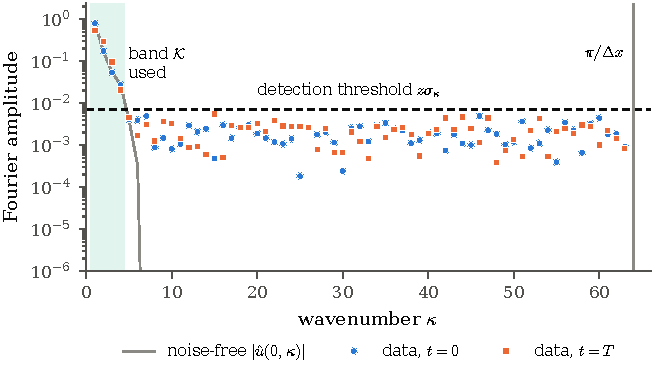
\includegraphics[width=0.66\linewidth]{fig_nyquist}
\caption{Fourier amplitudes of the worked example of \cref{sec:worked} (running example, grid, $5\%$ noise) at the first and last time, against the per-bin
detection threshold $z\,\sigbin$ ($z=3$). Only the shaded band of wavenumbers carries information
about the symbol; the spatial Nyquist limit $\pi/\Delta x$ is far away and is not the binding constraint.
What limits the band is the noise floor together with the decay of the diffusive modes
(\cref{sec:nyquist}).}\label{fig:nyquist}
\end{figure}

\paragraph{Wavenumbers per group}
The band must contain enough distinct wavenumbers on each branch for the factor to be determined.

\begin{proposition}[Counting condition]\label{prop:counting}
Let $Q=\tau-\Lambda(\xi)$ with $\Lambda$ a polynomial of degree at most $d$ with complex coefficients. The
coefficients are determined by the rates $\lambda(\kappa_\ell)=\Lambda(i\kappa_\ell)$ at $d+1$ distinct wavenumbers
$\kappa_\ell\in\R$, and not by fewer. The coefficient error is bounded by $\norm{\mathsf V^{-1}}\max_\ell\abs{\delta\lambda_\ell}$,
where $\mathsf V=\big((i\kappa_\ell)^k\big)$ is the Vandermonde matrix of the nodes; $\norm{\mathsf V^{-1}}$ grows like
$h_\kappa^{-d}$ when the nodes cluster, where $h_\kappa=\max_{\ell,\ell'}\abs{\kappa_\ell-\kappa_{\ell'}}$ is their spread. If the coefficients are real, the rates at
$-\kappa$ are the conjugates of those at $\kappa$, and $\lfloor d/2\rfloor+1$ distinct values of $\abs{\kappa}$ suffice,
at least $\lceil d/2\rceil$ of them nonzero.
\end{proposition}

\begin{proof}
$\Lambda(i\kappa)=\sum_{k\le d}\beta_k(i\kappa)^k$ is linear in $(\beta_0,\dots,\beta_d)$ with matrix $\mathsf V$,
which is invertible iff the $d+1$ nodes $i\kappa_\ell$ are distinct; with $d$ nodes a polynomial of
degree $d$ vanishing at all of them can be added. The bound is the norm of the inverse; for nodes
within $h_\kappa$ of each other the Lagrange basis polynomials have coefficients of size
$h_\kappa^{-d}$~\cite{Gau62}. For real $\beta_k$, $\operatorname{Re}\Lambda(i\kappa)=\sum_k(-1)^k\beta_{2k}\kappa^{2k}$ and
$\operatorname{Im}\Lambda(i\kappa)=\sum_k(-1)^k\beta_{2k+1}\kappa^{2k+1}$ separate the even and the odd coefficients, which are
polynomials in $\kappa^2$ with $\lfloor d/2\rfloor+1$ and $\lceil d/2\rceil$ unknowns.
\end{proof}

\roleinalg{The band $\mathcal K$ is the set of wavenumbers below both Nyquist limits whose amplitude
exceeds $z\,\sigbin$ (default $z=3$). A factor of degree $d_j$ in $\xi$ is reported as \FC{}
only if its modes occupy at least $d_j+1$ distinct signed wavenumbers $\kappa\in\mathcal K$ (for a real field the
modes at $\pm\kappa$ come in conjugate pairs, and the rule then implies the real-coefficient count of the proposition), and the whole band is
used rather than the cleanest few bins, because spreading the nodes is what keeps $\mathsf V$ well
conditioned. \Cref{fig:nyquist} shows the band for the running example.}

% Shared module: the outer loop over operator classes.
\subsection{The outer loop: choosing the class of operators}\label{sec:alg-loop}
A \emph{structure} $\Mfit=((m_1,d_1),\dots,(m_N,d_N))$ fixes the number $N$ of factors and, for each,
its degree $m_j$ in $\tau$ and $d_j$ in $\xi$; a factor is monic in $\tau$. For the running example the true structure is
$\Mfit=((1,1),(1,2))$: one factor of degree one in $\tau$ and one in $\xi$ ($\tau+c\xi$), and one of degree one in $\tau$
and two in $\xi$ ($\tau-\nu\xi^2$). The \emph{class} $\mathcal C(m,d)$ contains all structures with $\sum_jm_j\le m$ and
every $d_j\le d$. The starting class $\mathcal C(3,4)$ contains $((1,1),(1,2))$, but also, for instance, $((2,2))$ (a single
second-order factor, such as the wave operator $\tau^2-c^2\xi^2$) and $((1,0),(1,1),(1,1))$ (three first-order factors);
it has $90$ structures, and the largest class allowed, $\mathcal C(4,8)$, has $1353$. For each structure the core
(\cref{sec:alg-pencil,sec:alg-structfit}) returns fitted factors and a fit score.

\paragraph{Comparing structures} The structures are compared by the Bayesian information criterion
\begin{equation}\label{eq:bic}
  \mathrm{BIC}(\Mfit)=2n_{\rm m}\log\max\big(\chi^2/(2n_{\rm m}),\,1\big)+n_{\rm par}(\Mfit)\log(2n_{\rm m}),
\end{equation}
where $n_{\rm m}$ is the number of fitted modes (each complex rate gives two real data, hence $2n_{\rm m}$),
$n_{\rm par}(\Mfit)$ is the number of free coefficients of the structure, and
\[
  \chi^2=\sum_{p=1}^{n_{\rm m}}\min\big(r_{j(p)}(p)^2,\,9\big)
\]
measures how badly the fitted factors explain the observed modes, through the distance $r_j(p)$ of each mode to the
factor it is assigned to, in units of its standard deviation (\eqref{eq:vardist} in \cref{sec:alg-structfit}). If the
structure is right and the rate errors are circular complex Gaussian, each $r_j(p)^2$ is the squared modulus of a
standard complex Gaussian, exponentially distributed with mean one, so that, ignoring the cap, $\chi^2$ follows over
noise realizations approximately one half of a chi-squared distribution with $2n_{\rm m}-n_{\rm par}$ degrees of
freedom, and $\chi^2/(2n_{\rm m})$ is close to $\tfrac12$. The first term of~\eqref{eq:bic} penalizes a poor fit and the
second penalizes complexity; because of the floor $\max(\cdot,1)$, misfit is penalized only once it clearly exceeds what
the noise explains, and the criterion never rewards a fit that is better than the noise level, which would only be
fitting noise. The criterion is turned into a
probability over structures,
\begin{equation}\label{eq:bic-post}
  P(\Mfit\mid\text{data})\propto e^{-\mathrm{BIC}(\Mfit)/2},
\end{equation}
so that every structure receives a score that trades its fit against its number of coefficients.

\paragraph{Growing the class} The class is grown rather than fixed in advance. Starting from $(m,d)=(3,4)$, the
algorithm raises $m$ or $d$ by one when (a) most of the posterior mass~\eqref{eq:bic-post} is on structures labelled
\MIS{} or \IDK{} (\cref{sec:alg-labels}), or (b) an omnibus goodness-of-fit test rejects the current fit,
$\log_{10}p<-3$, where $p$ is the $p$-value of the test under the hypothesis that the fitted structure explains the data.
A larger class almost always fits better, simply because it has more degrees of freedom, so it is kept only if two
further checks pass. The \emph{held-out check} fits the modes of the earlier part of the time window and predicts those
of the later part: a structure that captures the dynamics predicts data it was not fitted to, while one that
only improves the fit to the data it has seen is overfitting. The \emph{mass-shift check} asks that the larger class
move posterior mass towards structures labelled \FC. Growth stops at $(4,8)$.

\paragraph{Regrouping} The loop runs on every field sample $u^{(1)},\dots,u^{(\Nsamp)}$, and different samples may give
slightly different answers: two factors in one sample and three in another, say. Coefficients of such answers cannot be
compared directly. The algorithm therefore takes the consensus structure, the one with the largest posterior mass over
all samples, and refits every sample at that structure (\emph{regrouping}); after this step every sample contributes one
fitted factor of each type, and factors from different samples can be compared and clustered (\cref{sec:bayes-cloud}).

This loop is the only ``regularization'' in the method, and it is a regularization of the
\emph{class}, by Occam's razor, not a penalty on coefficients. A Tikhonov or sparsity penalty would be
the wrong tool: it cannot make the interaction vanish (\cref{prop:discont}), and it can push the error of the split
below the unbiased floor $\noise^2/\gN$ (\cref{sec:limits}) only by shrinking the components towards a prior, which the
split layer of \cref{sec:bayes-split} does explicitly and reports.

% Shared module: matrix pencil per wavenumber.
\subsection{Reading the eigenvalues: the matrix pencil}\label{sec:alg-pencil}
For each sample field the spatial Fourier transform gives, for every $\kappa\in\mathcal K$, a time series
$\hat u(t_\ell,\kappa)$, $\ell=0,\dots,n_t-1$. For a constant-coefficient equation it is an exponential sum,
\begin{equation}\label{eq:expsum}
  \hat u(t,\kappa)=\sum_{p=1}^{r(\kappa)}A_p\,e^{\lambda_p(\kappa)t},\qquad Q_{j(p)}\big(\lambda_p,i\kappa\big)=0,
\end{equation}
one term per root of the symbol at that wavenumber. This step does \emph{not} fit the factors of the equation. It
extracts, at each wavenumber separately, the temporal rates $\lambda_p(\kappa)$, which are the eigenvalues of $\partial_t$
restricted to the finite-dimensional space spanned by the time series and its shifts, exactly as in \cref{lem:ep}.
Because every rate satisfies $Q_j(\lambda_p,i\kappa)=0$ for one factor, the factors are recovered afterwards by finding
the relation between $\lambda$ and $\kappa$, that is, the dispersion relation of each group (\cref{sec:alg-structfit}):
the search for the equation happens in frequency.

We compute the rates with the matrix pencil method~\cite{HuaSar90}. From the time series at one wavenumber form the Hankel matrix $H_{\ell k}=\hat u(t_{\ell+k},\kappa)$, whose columns are copies of the time series shifted by
one step each, and estimate the number of exponentials $r$ from its singular values. Let $Y_0$ be $H$ without its last
column and $Y_1$ be $H$ without its first column, both projected on the $r$ leading singular directions. Advancing a
time series by one step multiplies its term $A_pe^{\lambda_pt}$ by $\mu_p=e^{\lambda_p\Delta t}$, so $Y_1$ is $Y_0$ with
each exponential multiplied by its own $\mu_p$, and these factors are the eigenvalues of the pencil:
\begin{equation}\label{eq:pencil}
  \lambda_p=\frac{1}{\Delta t}\log\mu_p,\qquad \mu_p\in\operatorname{eig}\big(Y_0^{+}Y_1\big),
\end{equation}
followed by a least-squares fit of the amplitudes $A_p$. A bin is used only if its amplitude exceeds
$z\,\sigbin$, and the order $r$ is selected per bin by BIC among $r_0,r_0+1,r_0+2$. The uncertainty of each rate is
taken from the Cram\'er--Rao bound, the smallest variance that any unbiased estimator of $\lambda_p$ can reach at this
noise level. It depends on how sensitive the time series is to a change of each parameter: with $\mathsf J$ the
Jacobian of~\eqref{eq:expsum} with respect to all rates and amplitudes in the bin,
$\sigma_{\lambda,p}^2=\sigbin^2[(\mathsf J^H\mathsf J)^{-1}]_{pp}$. Rates of weak or quickly decaying modes, or of two modes with
nearly equal rates, are sensitive to noise and receive a large $\sigma_{\lambda,p}$.

The output is a cloud of points $(\kappa,\lambda_p(\kappa))$ with error bars. The modes of one group lie
on one branch of the dispersion relation; \cref{fig:directions} shows these branches for the
running example. Two rates closer than about $4/T$ cannot be resolved in a window of length $T$; such
a bin is flagged as \emph{confluent} and the factors involved are labelled \UND{} rather than forced
apart.

\begin{remark}[Variable coefficients and higher dimension]\label{rem:varcoef}
For constant coefficients the rates $\lambda_p(\kappa)$ do not depend on $x$; this is what allows one
spectral decomposition per wavenumber. If the coefficients vary slowly in $x$, a windowed transform
gives local rates $\lambda_p(\kappa;x_0)$, and each group becomes a \emph{family} of branches indexed by
$x_0$; the structured fit below would then regress coefficient functions instead of numbers. In $d$ space dimensions
the same construction applies with a wavenumber vector $\kappa\in\R^d$: the pencil still reads the temporal rates at
each $\kappa$, one small eigenvalue problem per wavenumber, and the groups become hypersurfaces $Q_j(\lambda,i\kappa)=0$
in $\C\times\C^d$. This makes the pencil a natural, though not necessarily the most efficient, first layer for
decomposing equations in higher dimension. What is missing is the second layer: a decomposition theorem for symbols in
$d+1$ variables, where two factors can share a whole curve of zeros and the overlap is no longer finite-dimensional.
Neither extension is implemented, and the algebraic guarantees of \cref{sec:factor} do not carry over unchanged
(for variable coefficients the ring becomes non-commutative).
\end{remark}

% Shared module: structured fit (grouping the modes into factors).
\subsection{Grouping the modes: the structured fit}\label{sec:alg-structfit}
The natural route, fitting one polynomial $P$ through all points $(\lambda_p,i\kappa_p)$ and then factoring
it, is ill-posed: a numerical polynomial with noisy coefficients is almost never reducible, and when it is
the factors move discontinuously with the coefficients. In our tests this route split the irreducible
Klein--Gordon and telegraph symbols into spurious factors at noise $10^{-4}$.

We group and fit at the same time. For a structure $\Mfit$ with $N$ factors we solve the
\emph{$N$-varieties} problem, a version of $k$-means clustering in which the cluster centres are curves instead of
points: assign every mode to the factor whose variety is nearest, refit each factor to the modes assigned to it, and
repeat the two steps until the assignment no longer changes (8 random starts, 30 iterations). The distance of a mode to factor $Q_j$ is
the first-order distance to its variety, scaled by the rate uncertainty,
\begin{equation}\label{eq:vardist}
  r_j(p)=\frac{\abs{Q_j(\lambda_p,i\kappa_p)}}{\sigma_{\lambda,p}\,\abs{\partial_\tau Q_j(\lambda_p,i\kappa_p)}},
\end{equation}
which plays the role of the Euclidean distance in $k$-means, and the misfit of a mode is $\min(r_j(p)^2,9)$; the cap makes isolated outliers count as a fixed
penalty instead of dragging a factor away. This is a clustering problem in which the clusters are
algebraic curves rather than points: the grouping of \cref{thm:factor} learned directly from the
spectrum.

% Shared module: recovering the components u_j, interference, recursion, labels, acceptance.
\subsection{Recovering the groups as functions}\label{sec:alg-components}
Once modes are assigned, the component of group $j$ is the sum of its modes,
\begin{equation}\label{eq:uj}
  u_j(t,x)=\sum_{p:\,j(p)=j}A_p\,e^{\lambda_p(t-t_0)+i\kappa_px},
\end{equation}
the discrete counterpart of the projector~\eqref{eq:lagrange}. A mode within distance $3$ of two
varieties lies in the overlap counted by $\deltaP$ (for the running example, the $\kappa=0$ mode); it is
split equally between the groups. This is the minimum-norm, or minimum-energy, choice among all splits allowed by
\cref{thm:factor}: if the shared mode has amplitude $A$ and is given as $\alpha A$ to one group and $(1-\alpha)A$ to the
other, the energy it adds to the components is $\abs{A}^2\big(\alpha^2+(1-\alpha)^2\big)$, which is smallest at
$\alpha=\tfrac12$. The data cannot tell the splits apart, so the algorithm takes the one that puts the least energy
into the ambiguity. It coincides with the posterior mean of the Bayesian layer (\cref{sec:bayes-split}), so the
convention is not arbitrary. The energy shares $w_j$ of~\eqref{eq:energy}
are computed from these components.

\subsection{Interference between groups and the recursion over components}\label{sec:alg-interference}
The groups are not orthogonal. Let $B_j$ be an orthonormal basis of the sampled kernel of $Q_j$ (all
exponentials $e^{\lambda t+i\kappa x}$ with $Q_j(\lambda,i\kappa)=0$, $\kappa\in\mathcal K$, on the grid) and
$\sumop=[B_1\cdots B_N]$. Then $\gN$ is the smallest eigenvalue of $\sumop^H\sumop$ above $10^{-8}$, the
eigenvalues below that threshold count the directions shared by two groups, and for two groups
$\gamma_2=1-\cF$. Because pairwise angles do not determine $\gN$ for $N\ge3$ (\cref{sec:cond}), the full
Gram matrix is used.

Each component $u_j$ is then analysed again by the same procedure, up to depth two: a factor that still
splits on its own component is replaced by its children. A split is accepted without further evidence
if it leaves the kernel unchanged, and otherwise only if it improves the evidence of \cref{sec:alg-accept} by more
than one nat. Complex factors of a real field are always kept together with their conjugates. The beam equation of
\cref{app:cases} is an example. The core first fits it as one factor of degree two in $\tau$,
$\tau^2+0.0903\,\xi^4$, whose component $u_1$ contains, at every wavenumber, two modes with rates
$\lambda=\pm0.30\,i\kappa^2$. The recursion finds that this factor splits along its two root branches, into the children
$\tau-0.3004\,i\xi^2$ and $\tau+0.3004\,i\xi^2$; their kernels together are the kernel of the parent, so the split is
accepted without further evidence, and the two children, which are complex conjugates, are reported together.

\subsection{Identifiability and the output labels}\label{sec:alg-labels}
\Cref{sec:certify} rules out the label ``identified''. Each reported structure carries one of four labels.
\begin{description}[leftmargin=2.9cm,labelwidth=2.7cm]
  \item[\FC] Every factor $Q_j$, of degree $m_j$ in $\tau$ and $d_j$ in $\xi$, has at least $m_j(d_j+1)+1$ modes
  (more data than coefficients), modes at $d_j+1$ distinct wavenumbers (\cref{prop:counting}), and $m_j$ modes
  at some single wavenumber (one per root); and the fit passes the goodness-of-fit test below.
  The data are compatible with the factored equation and pin down its coefficients within the class.
  \item[\IDK] The fit is good, but some factor is determined only relative to the declared class (too
  few distinct wavenumbers): another equation of a larger class fits equally well.
  \item[\MIS] The goodness-of-fit test rejects the structure.
  \item[\UND] The data cannot decide, typically because of confluent rates or a repeated factor.
\end{description}
Repeated factors ($Q=P_i^2$) are always reported as \UND: by \cref{thm:ident}(b) a repeated factor is
visible only through polynomial prefactors $t\,e^{\lambda t}$, which finite noisy data cannot separate from
two nearby rates.

\subsection{Noise level and acceptance}\label{sec:alg-accept}
The noise level enters in three places. The observation noise $\noise$ is integrated out in the
interpolation (\cref{sec:alg-interp}). Per Fourier bin it becomes $\sigbin$, which sets the band and the
rate uncertainties. In the final decision it is used against the \emph{raw observations}, not against the
interpolated field. A candidate set of factors $Q_1,\dots,Q_N$ defines a linear model for the vector $y$ of the $n$
observations: let $E_j$ be the matrix whose columns are the exponentials $e^{\lambda t+i\kappa x}$ of the kernel of $Q_j$
(the functions spanned by $B_j$ in \cref{sec:alg-interference}), evaluated at the observation points, $E=[E_1\cdots E_N]$,
and let $a$ be the vector of their amplitudes. Then
\[
  y=Ea+\varepsilon,\qquad \varepsilon\sim\Normal(0,\noise^2I),\qquad a\sim\Normal(0,\omega^2I),
\]
where $I$ is the identity matrix, so that $\noise^2I$ and $\omega^2I$ are the covariance matrices of the noise and of the
amplitudes, and $\omega^2$ is the prior variance of each amplitude. Both are multivariate Gaussian distributions, and
integrating the amplitudes out gives the distribution of the data under the candidate,
\[
  y\mid Q_1,\dots,Q_N\ \sim\ \Normal\big(0,\ \noise^2I+\omega^2EE^H\big),
\]
with $E^H$ the conjugate transpose of $E$. The score of the candidate adds a complexity penalty to the logarithm of
this density,
\begin{equation}\label{eq:raw-evidence}
  S(Q_1,\dots,Q_N)=\log\Normal\big(y;\,0,\ \noise^2I+\omega^2EE^H\big)-\tfrac12\,n_{\rm par}\log n ,
\end{equation}
where $n_{\rm par}$ is the number of coefficients that define the factors. The first term is the log-probability of
the observations actually made under the candidate factors, with the amplitudes integrated out; the second, as in the
Bayesian information criterion, approximately accounts for the coefficients of the factors themselves, which were fitted
rather than integrated, and penalizes candidates with more of them.
The score is built to \emph{compare} candidate structures on the same data, which of two factor sets explains the
observations better, not to judge one fit in isolation. It decides between candidates: dropping a factor, dropping a term whose $90\%$
interval contains zero, merging two factors, or splitting one. A change is accepted only if it gains more
than one nat. The same model gives a goodness-of-fit test: with $\hat y$ the projection of $y$ on the columns of $E$,
\[
  \chi^2=\sum_{i=1}^{n}\frac{\abs{y_i-\hat y_i}^2}{\noise^2},
\]
which, if the candidate is right and the noise Gaussian (variance $\noise^2$ per real observation), approximately follows
a chi-squared distribution over noise realizations with $n-\rank E$ degrees of freedom; $\rank E$ rather than the number of
columns, because a mode shared by two groups appears in both $E_1$ and $E_2$, and only approximately, because the rates in
$E$ were themselves fitted to the data. (For complex data with $\mathbb E\abs{\varepsilon_i}^2=\noise^2$ the statistic is half
a chi-squared variable with $2(n-\rank E)$ degrees of freedom.) A $p$-value below $10^{-3}$
turns the label into \MIS. Deciding on the raw data matters:
the interpolant has already smoothed the high wavenumbers, and a candidate that fits the interpolant may
not fit the observations.

Finally the interaction ratio $\rho$ of~\eqref{eq:energy} is computed for every evolution factor (degree one in $\tau$) with more than one
term from the closed form~\eqref{eq:eint-fourier}. It is reported, not used to accept or reject: by
\cref{prop:discont} it is a diagnostic of the evolution inside a factor, not a test of the factor.


\section{The statistical layer}\label{sec:bayesian}
The deterministic core gives one answer per field sample. The statistical layer turns the answers for all samples
into one distribution. It has two parts: a Gaussian model of the components given the factors, which converts the
Friedrichs angle into credible intervals, and a clustering of the factors found in all samples, which decides how
many groups there are and what they are.
% Shared module: the statistical layer (split layer, cloud, Dirichlet-process clustering, decision).
\subsection{Gaussian prior on the components and the split layer}\label{sec:bayes-split}
The core returns factors and components for one field. The first statistical question is how well the
components are determined given the factors. On the observation window write
\begin{equation}\label{eq:linmodel}
  u=\sum_{j=1}^NB_ja_j+\varepsilon=\sumop a+\varepsilon,\qquad \varepsilon\sim\Normal(0,\noise^2I),\qquad a\sim\Normal(0,\omega^2I),
\end{equation}
with $B_j$ the orthonormal kernel bases of \cref{sec:alg-interference} and $a_j$ the coefficients of component $j$ in
that basis. As in \cref{sec:alg-accept}, $\omega^2$ is the prior variance of each coefficient, now in the orthonormal
basis: the prior covariance of $a$ is the diagonal matrix $\omega^2I$. This Gaussian prior on the \emph{coefficients of the components} is the second
prior of the method; the first, in \cref{sec:alg-interp}, is on the field. Given the data, the coefficients are again
Gaussian, centred at the regularized least-squares fit and with covariance $\Gamma_a$:
\begin{equation}\label{eq:postcov}
  a\mid u\ \sim\ \Normal\big(\hat a,\Gamma_a\big),\qquad
  \hat a=\Big(\sumop^H\sumop+\frac{\noise^2}{\omega^2}I\Big)^{-1}\sumop^Hu,\qquad
  \Gamma_a=\noise^2\Big(\sumop^H\sumop+\frac{\noise^2}{\omega^2}I\Big)^{-1}.
\end{equation}
The layer therefore does not return one split of $u$ but a Gaussian distribution of splits around the fitted one.

\begin{proposition}[The angle sets the error bars]\label{prop:bayes-angle}
For two groups the eigenvalues of $\sumop^H\sumop$ are $1\pm\cos\theta_k$, with $\theta_k$ the principal
angles between the sampled kernels, together with the eigenvalue $1$ of multiplicity
$\abs{\dim M_1-\dim M_2}$. In the worst direction orthogonal to $\ker\sumop$ the posterior variance of the component
coefficients is
\begin{equation}\label{eq:worstvar}
  \frac{\noise^2}{\gamma_2+\noise^2/\omega^2},\qquad \gamma_2=1-\cF .
\end{equation}
On the shared directions ($\theta_k=0$, the overlap $\deltaP$) the likelihood is flat, the posterior equals
the prior, and the posterior mean splits the shared part equally.
\end{proposition}

\begin{proof}
With orthonormal $B_1,B_2$, $\sumop^H\sumop=\begin{psmallmatrix}I&B_1^HB_2\\B_2^HB_1&I\end{psmallmatrix}$; the singular
values of $B_1^HB_2$ are the $\cos\theta_k$, which gives the eigenvalues $1\pm\cos\theta_k$ (and $1$ on the
directions of the larger space without a partner), and \eqref{eq:postcov} is diagonal in the same basis. The
smallest nonzero eigenvalue $1-\cF$ gives
\eqref{eq:worstvar}. For $\theta_k=0$ the likelihood depends on $a_1+a_2$ along that direction only, so
the posterior along $a_1-a_2$ is the prior, centred at zero; its variance there is $\omega^2$.
\end{proof}

Equation~\eqref{eq:worstvar} is the Bayesian form of the stability bound~\eqref{eq:stability}: credible
intervals grow like $\noise/\sin(\thetaF/2)$ as the angle closes, and are capped by the prior when
$\thetaF\to0$. The scale $\omega^2$ is not set by hand: it is the value that makes the observed field most probable
(empirical Bayes),
\[
  \hat\omega^2=\operatorname*{arg\,max}_{\omega^2}\ \log\Normal\big(u;\,0,\ \noise^2I+\omega^2\sumop\sumop^H\big),
\]
maximized over a grid from $10^{-6}$ to $10^{2}$. The same evidence compares the model
$u\in M_1\oplus M_2$ with the model with one factor, which gives the probability $P(\text{split})$; as
$\thetaF\to0$ the evidence ratio tends to one and $P(\text{split})$ returns to its prior. The energy shares $w_j$ are nonlinear functions of $a$, so their intervals are
obtained by Monte Carlo, without linearization: the layer draws $400$ coefficient vectors $a^{(1)},\dots,a^{(400)}$ from
the Gaussian~\eqref{eq:postcov}, computes the shares of each, and reports their quantiles.

\subsection{Many samples, one cloud: grouping across samples}\label{sec:bayes-cloud}
The core runs on each of the $\Nsamp$ posterior field samples $u^{(q)}$ of \cref{sec:alg-interp}. Every sample
returns its own factors, with energy shares $w_j^{(q)}$. The same physical group appears once per sample, with slightly different
coefficients, and sometimes split into two near-copies or merged with a neighbour. The second grouping
problem is therefore to recognize the same factor across samples.

Each factor is mapped to a point of a fixed coefficient space: the monic coefficient vector
$\beta\in\C^{m\times(d+1)}$ of its symbol, zero-padded to the largest degrees in play, so that equal
operators give equal vectors whatever their position in a sample's list. The \emph{cloud} is the weighted
point measure
\begin{equation}\label{eq:cloud}
  \cloud=\sum_{q=1}^{\Nsamp}\pi_q\sum_jw_j^{(q)}\,\delta_{\beta_j^{(q)}},
\end{equation}
which gives each factor the mass of its sample times its energy share. Here $\pi_q$ is the weight of the field
sample $u^{(q)}$, inherited from the marginalization over the Gaussian-process hyperparameters~\eqref{eq:marginal-eta};
$w_j^{(q)}$ is the energy share~\eqref{eq:energy} of factor $j$ in that sample, computed from the components of that
sample (one value per factor and sample, not an average over the Monte Carlo draws above); and $\delta_{\beta}$ is a unit
point mass at the coefficient vector $\beta$, so that each factor appears in the cloud as one point. A sharp equation is a cloud with
a few tight clusters; an uncertain one is a diffuse cloud.

\paragraph{Dirichlet-process clustering}
Each group of points in the cloud is modelled as a Gaussian cluster around the coefficient vector of its factor, so
the cloud as a whole is described by a Gaussian mixture model (GMM): a weighted sum of Gaussian densities, one per
group, with weights given by the cluster masses. A finite GMM needs the number of groups in advance. The number of
groups is not known, so we use its Dirichlet-process version, which lets the data choose it: a Dirichlet-process Gaussian mixture
(truncated stick-breaking with eight mixture atoms, diagonal covariances, variational
inference~\cite{BleJor06}), separately for each degree $m$ in $\tau$. The concentration $\alpha$ is chosen
on the grid $\{10^{-3},\dots,10\}$ by the evidence lower bound. Each factor enters the fit once plus a
number of copies proportional to its mass; replicating every factor many times instead splits one group
into several clusters. Two clusters that never occur together in the same sample are merged when a
full-covariance BIC prefers one Gaussian; full covariances are needed because coefficients of one factor
are strongly correlated (in the worked example of \cref{sec:worked}, the constant and the $\xi^2$ coefficient of the diffusion factor
have correlation $0.78$ across 32 samples).

\paragraph{The final distribution}
The output is a distribution, not a point estimate:
\begin{itemize}
  \item the factors (cluster centres) with $90\%$ intervals for every coefficient (quantiles over posterior samples, or over
  parametric-bootstrap refits on gridded input);
  \item the posterior $P(k)$ of the number $k$ of groups, by Monte Carlo over samples and cluster
  responsibilities, together with the posterior over structures from~\eqref{eq:bic};
  \item the energy shares $w_j$ with intervals, $P(\text{split})$, $\gN$, $\cF$ and the distribution of $\rho$;
  \item the label of \cref{sec:alg-labels}.
\end{itemize}
The effective number of groups $\keff=\exp(-\sum_j\bar w_j\log\bar w_j)$, with $\bar w_j$ the cluster masses, is reported
but never rounded to decide $k$: rounding is fragile (a spurious mass of $1.4\%$ moves $\keff$ from $2.00$ to
$2.13$), so $k$ is read from $P(k)$.

\paragraph{When is the model good enough?}
The decision combines four quantities, in this order: the raw-data goodness of fit (otherwise \MIS); the
concentration of $P(\Mfit)$ on one structure (at least $0.9$) and of $P(k)$ on one value; the counting
condition of \cref{prop:counting} (otherwise \IDK); and the conditioning, read through $\gN$ and
$P(\text{split})$. A small Friedrichs angle does not reject the equation, it widens the intervals of the
components and lowers $P(\text{split})$. The reader therefore always sees how well each group is
separated from the others, not only whether the equation fits.


\section{Results}\label{sec:results}
We test the method in three ways. \Cref{sec:worked} follows one data set through every stage, so that each quantity of
the output can be seen and interpreted. \Cref{sec:bench} compares the method with library regression and dynamic mode
decomposition on a benchmark of ten equations in three designs, and evaluates it on twenty random equations that were
not used in its development.
% Shared module: the worked example (one complete run).
\subsection{A complete run on one data set}\label{sec:worked}
We follow one input through every stage. The data are the running example (\cref{ex:tpd}) with $c=1$,
$\nu=0.3$, observed on a $64\times128$ grid over $[0,2]\times[0,2\pi)$ with white noise of standard deviation
$\noise=0.05\,\mathrm{std}\abs u$, the hardest grid setting of the benchmark in \cref{sec:bench}. The pipeline is
run exactly as in the benchmark: one noisy grid, the outer loop with default parameters, and $16$
parametric-bootstrap refits for the intervals. The run takes about two minutes on one core.
The figures of this subsection also use a second run on the same input with $\Nsamp=32$ posterior samples,
which shows the cloud of \cref{sec:bayes-cloud}.

\paragraph{The band} Of the 64 positive wavenumbers below $\pi/\Delta x=64$, only $\kappa\le4$ rise above the
detection threshold (\cref{fig:nyquist}); the noise-free field has negligible energy beyond $\kappa\approx5$, and
a diffusive mode at $\kappa=3$ loses a factor $e^{-0.3\cdot9\cdot2}\approx e^{-5.4}$ of its amplitude over the
window. Every later decision is made with these few bins.


\paragraph{Modes and directions} The matrix pencil returns twelve modes (\cref{fig:directions}). Eight lie on
the line $\operatorname{Im}\lambda=-\kappa$ with $\operatorname{Re}\lambda\approx0$ (transport), four on the parabola
$\operatorname{Re}\lambda=-0.3\kappa^2$ with $\operatorname{Im}\lambda\approx0$ (diffusion). Each factor is a
\emph{direction} in the frequency plane: a curve along which its modes line up. The structured fit
recovers the two curves; the thin lines are the factors fitted to the 32 posterior samples and show the
uncertainty of each curve, larger for diffusion at high $\abs\kappa$, where there are no modes. The counting
condition of \cref{prop:counting} holds: the transport modes occupy eight distinct wavenumbers
($\kappa=\pm1,\dots,\pm4$) and the diffusion modes four ($\pm1,\pm2$), against the two and three required
for factors of degree one and two in $\xi$.

\emph{How \cref{fig:directions} is built.} Each point is one mode $(\kappa,\lambda)$ returned by the pencil: its
horizontal position is the wavenumber, its height the oscillation $\operatorname{Im}\lambda$ (panel a) or the damping
$\operatorname{Re}\lambda$ (panel b), and its colour the factor to which the structured fit assigned it. Each thin line is
one fitted factor, drawn as its dispersion curve $\lambda=\Lambda_j(i\kappa)$ for all $\kappa$, one line per factor and
posterior sample. In the figure, the transport group is a sloped line in (a) and a flat line at zero in (b), a mode
that travels without decaying; the diffusion group is flat in (a) and a downward parabola in (b), a mode that does not
travel and decays faster at higher wavenumber. The thin lines bundle tightly where there are modes and fan out where
there are none.

\begin{figure}[tbp]
\centering
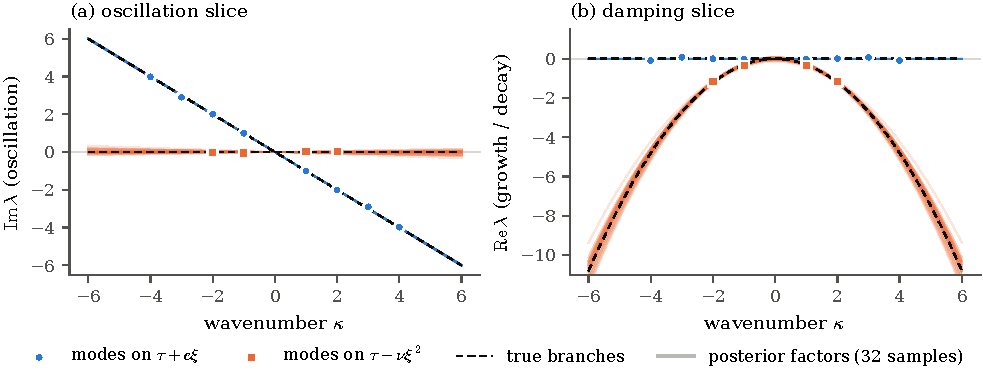
\includegraphics[width=\linewidth]{fig_directions}
\caption{The two groups of the running example as directions in the frequency plane. Points: modes found
by the matrix pencil in the noisy data, coloured by the factor they were assigned to. Dashed: the true
dispersion branches $\lambda=-ic\kappa$ and $\lambda=-\nu\kappa^2$. Thin lines: the factors fitted to 32
posterior samples of the same input; their spread is the uncertainty of each direction. The points come from the run
with the benchmark protocol, the lines from the 32-sample run. (a) Oscillation, $\operatorname{Im}\lambda$;
(b) damping, $\operatorname{Re}\lambda$.}\label{fig:directions}
\end{figure}

\paragraph{Grouping and the evidence step} At the starting class the data-level evidence ranks the
structure $((1,1),(1,2))$ (one factor of degree $(1,1)$, one of degree $(1,2)$) first, $0.13$ nats ahead of
$((1,1),(1,3))$; the second class contains the first, so both are compatible with the truth and the simpler
one is kept. The core, applied to the noisy grid, initially returned \emph{three} factors: the diffusion
factor and two near-copies of the transport factor, $\tau+1.0006\,\xi$ and $\tau+1.0044\,\xi-0.0028$. Grouping
by evidence on the observations removed the duplicate (the factor set without it has higher evidence), and
dropped the constant terms, whose intervals contained zero. An earlier version of the pipeline (the row ``previous version'' of \cref{tab:bench}) returned a similar triple on
this input, two transport copies $\tau+0.9989\,\xi$ and $\tau+1.0044\,\xi$ and a diffusion factor $\tau-0.263\,\xi^2$, and
labelled it \FC: a confident wrong answer that the grouping step now prevents.

\paragraph{Cloud and clusters} Over 32 posterior samples the core returns 64 factors. In coefficient space
they form two tight clusters around the true factors (\cref{fig:grouping}a), and the largest principal angle
between their kernels is near zero inside a cluster and about $1.2$ rad across clusters
(\cref{fig:grouping}b). The Dirichlet-process mixture finds two clusters with masses $0.767$ and $0.233$;
$P(k=2)=1$ and $\keff=1.72$ ($90\%$ interval $[1.67,1.79]$), which is far from $2$ only because the two
groups carry unequal energy.

\emph{How \cref{fig:grouping} is built.} In panel (a) each marker is one factor found in one posterior sample,
placed at its coefficient of $\xi$ (horizontal) and of $\xi^2$ (vertical), with area proportional to its mass in the
cloud. Panel (b) compares every pair of these factors by the spaces of functions they allow: for each factor we take the
span of its kernel exponentials on the grid and band, and compute the principal angles between the two spans from the
singular values of $B_i^HB_j$ (their cosines). The colour shows the largest of these angles, light for nearly
the same space and dark for very different spaces, with rows and columns ordered by cluster. The figure shows, in (a),
two tight, well separated clouds and nothing in between; in (b) two light blocks on the diagonal, because all factors of
one group allow the same functions, and dark blocks off the diagonal, because the two groups do not. (The largest angle
is used here to tell kernels apart; the Friedrichs angle of \cref{sec:cond} is the smallest nonzero one, which measures
how well two different groups can be separated.)

\begin{figure}[tbp]
\centering
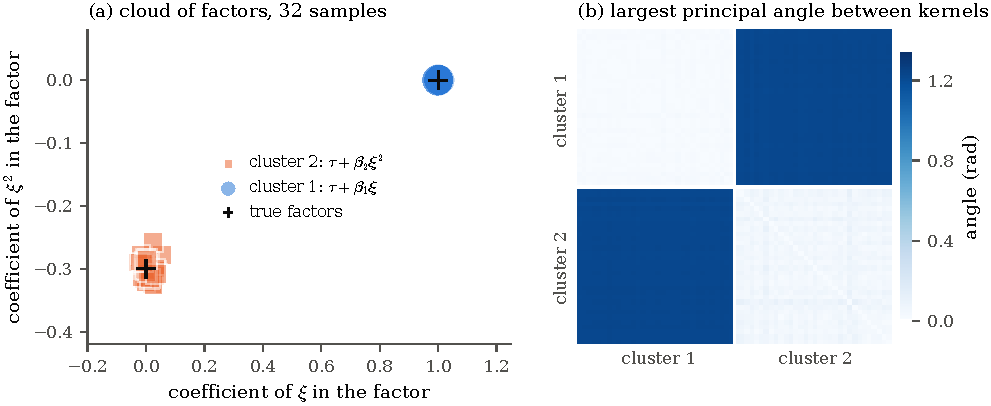
\includegraphics[width=\linewidth]{fig_grouping}
\caption{Grouping across posterior samples. (a) Each marker is one factor returned for one of 32 posterior
samples, placed by its coefficients of $\xi$ and $\xi^2$, the two that separate the groups; area is proportional to its mass $\pi_qw_j$; crosses mark the true
factors. (b) Largest principal angle between the sampled kernels of every pair of factors, ordered by cluster:
the block structure is the grouping.}\label{fig:grouping}
\end{figure}

\paragraph{Components and energy} \Cref{fig:components} shows the data, the two components and the residual.
The transport group carries $w_1=0.768$ of the energy and the diffusion group $w_2=0.232$, with $90\%$
intervals of width below $0.002$. The joint residual of the data on the two kernels is $2.5\%$ of the data
norm, and it shows no structure (\cref{fig:components}d). Each reported factor has a single term besides $\partial_t$, so its
interaction ratio is $\rho=0$ by definition. Computed on the factors of the cloud before pruning, $\rho$ has median $0.03$
($90\%$ interval $[0.01,0.07]$ over 32 samples), entirely due to the small constant and $\xi$ coefficients that
the evidence step removes. For comparison, on the advection--diffusion equation (one factor with the two
terms $c\partial_x$ and $\nu\partial_x^2$) the same pipeline reports $\rho=0.79$, with a $90\%$ interval
$[0.788,0.793]$ over 16 samples: there the interaction is most of the evolution, as \cref{thm:eint} predicts.

\emph{How \cref{fig:components} is built.} Each panel is a map of a function of $(t,x)$, with $x$ horizontal and $t$
vertical, red for positive and blue for negative values, on one colour scale for all panels. The components are the sums
of the modes of each group, \eqref{eq:uj}. The transport component consists of tilted stripes, a profile
that moves at speed $c=1$ without changing shape; the diffusion component has vertical structure that fades with time; the
residual has no pattern left.

\begin{figure}[tbp]
\centering
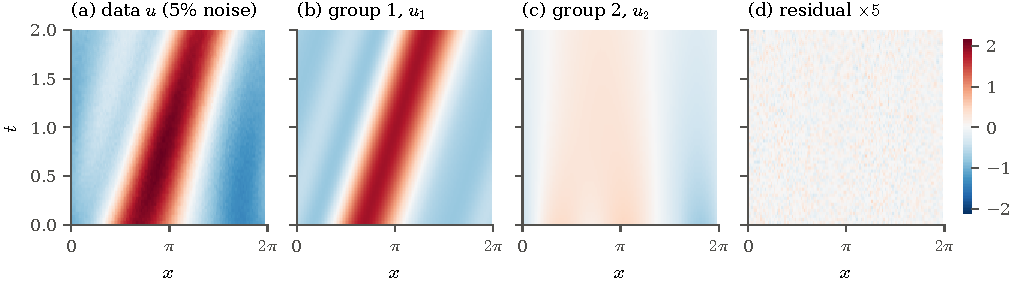
\includegraphics[width=\linewidth]{fig_components}
\caption{The data of the worked example and its two groups as functions of $(t,x)$, on a common colour scale:
(a) noisy data; (b) transport component; (c) diffusion component; (d) residual, magnified five times, which
is indistinguishable from the noise.}\label{fig:components}
\end{figure}

\paragraph{The output} \Cref{tab:worked} lists the final output and how to read it. The separation of the two
groups is moderate: $\cF=0.827$, $\thetaF=0.60$ rad, so errors in the components are amplified by at most
$\gN^{-1/2}=2.41$. For contrast, the two conjugate factors of the beam equation
$\tau\mp0.3\,i\xi^2$ (\cref{app:cases}) are recovered with the same accuracy but are much closer to each other: $\cF=0.939$, an
amplification of $4.05$.

\begin{table}[tbp]
\centering\small
\caption{Output of the worked example and how to read each quantity. Intervals are $90\%$ intervals
from 16 parametric-bootstrap refits.}\label{tab:worked}
\begin{tabularx}{\linewidth}{@{}l l X@{}}
\toprule
Quantity & Value & Meaning\\
\midrule
equation & $(\tau+1.0006\,\xi)(\tau-0.2980\,\xi^2)$ & recovered factors; truth $(\tau+\xi)(\tau-0.3\,\xi^2)$, largest relative error $0.7\%$\\
coefficient of $\xi$ & $1.0006\ [0.9998,1.0020]$ & speed $c$ of the transport group\\
coefficient of $\xi^2$ & $-0.2980\ [-0.3049,-0.2919]$ & diffusivity $\nu$ of the diffusion group\\
label & \FC & enough distinct wavenumbers per factor, goodness of fit passed\\
$P(k)$ & $P(k=2)=1$ & posterior over the number of groups\\
$w_1,\ w_2$ & $0.768,\ 0.232$ & energy shares~\eqref{eq:energy} of the two groups\\
$P(\text{split})$ & $1.000$ & evidence that the data need both groups\\
$\gN,\ \cF,\ \thetaF$ & $0.173,\ 0.827,\ 0.60$ & separation of the groups (\cref{sec:cond})\\
$\gN^{-1/2}$ & $2.41$ & worst-case error amplification of the components\\
$\rho$ & $0$ & no interaction inside either reported factor (single terms)\\
\bottomrule
\end{tabularx}
\end{table}

% Shared module: benchmarks.
\subsection{Benchmarks}\label{sec:bench}
\paragraph{Design} The benchmark has ten linear constant-coefficient equations in one space dimension:
transport, heat, advection--diffusion, Airy, Schr\"odinger (complex field), beam, wave, Klein--Gordon,
telegraph, and the running example. Each is observed in three designs: a $64\times128$ grid with noise
$1\%$, the same grid with noise $5\%$, and $400$ scattered points with noise $5\%$ (noise standard deviation
relative to $\mathrm{std}\abs u$). This gives $30$ inputs. We compare with weak SINDy, ensemble SINDy,
SBR SINDy~\cite{MesBor21,FasKutBru22,HirBarKut22}, PDE-FIND~\cite{RudBruProKut17} and BOP-DMD~\cite{SasKut22}, each
run on the same input (on the scattered designs, on the same interpolated field) through the reference
implementations PySINDy and PyDMD. The SINDy variants use a linear library of mixed derivatives, a target
$\partial_t^{\,m}u$ of every order the benchmark needs, and a sparsity threshold selected by BIC over a grid
of fourteen values (zero and $10^{-4},\dots,1$); their answers are therefore tuned to the same linear class as ours. An answer is \emph{right} if the recovered set of factors matches the true one
within relative coefficient error $0.05$; \emph{equivalent} if it is the same product polynomial written
differently; an \emph{abstention} if the method declines (labels \IDK{} or \UND); and
\emph{false-confident} if it returns a wrong equation as if it were right. The baselines have no way to
abstain, so every wrong baseline answer is false-confident.

\begin{figure}[tbp]
\centering
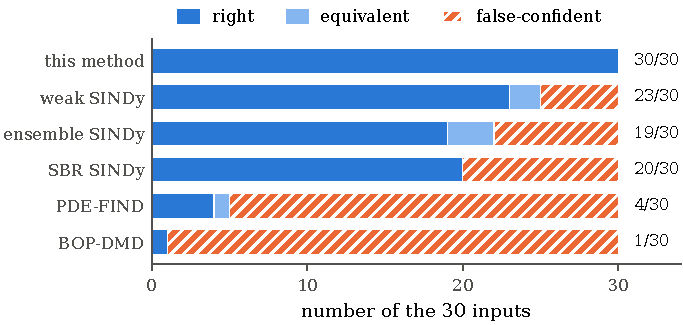
\includegraphics[width=0.7\linewidth]{fig_bench}
\caption{Outcomes on the 30 benchmark inputs (10 equations $\times$ 3 designs). Hatched: false-confident
answers, i.e.\ a wrong equation returned without any warning.}\label{fig:bench}
\end{figure}

\begin{table}[tbp]
\centering\small
\caption{Benchmark outcomes per design (right or equivalent / false-confident, out of 10 each) and coefficient
coverage. ``Previous version'' is an earlier run of the same pipeline with earlier decision rules. Runtimes are wall-clock medians per input; the pipeline ran
with several workers on a shared machine.}\label{tab:bench}
\begin{tabular}{@{}lcccccc@{}}
\toprule
Method & grid 1\% & grid 5\% & 400 pts 5\% & total & coef.\ cover$_{90}$ & median time\\
\midrule
this method        & 10 / 0 & 10 / 0 & 10 / 0 & 30 / 0 & 0.94 & 127 s\\
previous version   & 10 / 0 & \phantom{1}8 / 1 & \phantom{1}8 / 0 & 26 / 1 & 0.84 & 5 s\\
weak SINDy         & 10 / 0 & \phantom{1}7 / 3 & \phantom{1}8 / 2 & 25 / 5 & -- & 3 s\\
ensemble SINDy     & \phantom{1}9 / 1 & \phantom{1}7 / 3 & \phantom{1}6 / 4 & 22 / 8 & -- & 5 s\\
SBR SINDy          & \phantom{1}8 / 2 & \phantom{1}6 / 4 & \phantom{1}6 / 4 & 20 / 10 & -- & 14 s\\
PDE-FIND           & \phantom{1}1 / 9 & \phantom{1}1 / 9 & \phantom{1}3 / 7 & \phantom{1}5 / 25 & -- & 0.6 s\\
BOP-DMD            & \phantom{1}1 / 9 & \phantom{1}0 / 10 & \phantom{1}0 / 10 & \phantom{1}1 / 29 & -- & 1.5 s\\
\bottomrule
\end{tabular}
\end{table}

\paragraph{Results} The method returns the right factor set on all $30$ inputs and is never
false-confident (\cref{fig:bench,tab:bench}). The best baseline, weak SINDy, is right or equivalent on $25$
and false-confident on $5$: the beam equation and the running example in two designs each, and the
Schr\"odinger equation on the grid at $5\%$ noise. Four of the five are products of factors (the wave equation, also a
product, is handled correctly by weak SINDy); the other SINDy variants fail on the same products and on further
inputs. Where the method returns intervals, the true coefficients fall inside the $90\%$ intervals in
$94\%$ of cases, and the true energy shares fall inside their intervals in all six inputs where a split was reported. The comparison with the previous version isolates the effect of the grouping decisions of
\cref{sec:alg-accept}: its one false-confident answer is the duplicated transport factor of
\cref{sec:worked}.

\paragraph{Independent repetitions} Because the $30$ inputs above share one field and one noise draw per equation,
we repeated the two grid designs with three further seeds, each drawing a new field \emph{and} a new noise
realization: $10$ equations $\times$ $2$ noise levels $\times$ $3$ seeds, $60$ independent inputs. \Cref{tab:multiseed}
compares the method with weak SINDy, the strongest baseline of \cref{tab:bench}. The method returns the right factor
set with the label \FC{} on all $60$ inputs, with coefficient coverage $0.94$ at nominal $0.90$; weak SINDy is
false-confident on $13$, again mostly on products of factors (the running example $5$ times, the beam twice) and on the
Schr\"odinger equation. With $60$ independent trials and no failure, a one-sided $95\%$ upper bound on the method's
false-confident rate on these designs is $5\%$.

\begin{table}[tbp]
\centering\small
\caption{Grid designs repeated with independent fields and noise (seeds $1$--$3$): right / false-confident out of $30$
per noise level. The weak-SINDy rows were rerun here with PySINDy~2.1.0 and the settings of \cref{tab:bench}.}\label{tab:multiseed}
\begin{tabular}{@{}lccc@{}}
\toprule
Method & grid 1\% & grid 5\% & total\\
\midrule
this method & 30 / 0 & 30 / 0 & 60 / 0\\
weak SINDy  & 26 / 4 & 21 / 9 & 47 / 13\\
\bottomrule
\end{tabular}
\end{table}

\paragraph{Equations outside the benchmark list} To test generalization we drew $20$ random equations
from five families: first-order factors (F1), first-order dispersive factors (F2), irreducible
second-order factors (F3), products of two or three factors (F4), and third-order factors or a reaction
factor times a transport factor, often with few excited wavenumbers (F5). None of these draws was used to
set any parameter. Each is observed on the grid
with $1\%$ noise. \Cref{tab:e13} reports the outcomes. ``Equivalent'' here means that the returned
equation explains the data as well as the true one by a $\chi^2$ test adjusted for degrees of freedom, and
``abstain-ok'' that the method abstained on an input that is genuinely not resolvable at this noise level:
a factor is resolvable when, computed from the truth alone, it has modes above the detection threshold at
$d_j+1$ distinct $\abs\kappa$ (a stricter count than the label rule of \cref{sec:alg-labels}) and each of its terms moves some visible rate by more than three standard deviations.

\begin{table}[tbp]
\centering\small
\caption{Twenty random equations from five families, grid, $1\%$ noise. ``Core'' is the deterministic core of
\cref{sec:alg-pencil,sec:alg-structfit} run once, without the outer loop and the statistical layer.}\label{tab:e13}
\begin{tabular}{@{}lcccccc@{}}
\toprule
Method & right & equivalent & abstain-ok & abstain & false-confident\\
\midrule
this method    & 12 & 7 & 1 & 0 & \phantom{1}0\\
core only      & \phantom{1}5 & 3 & 3 & 3 & \phantom{1}6\\
ensemble SINDy & \phantom{1}6 & 1 & 0 & 0 & 13\\
weak SINDy     & \phantom{1}5 & 1 & 0 & 0 & 14\\
PDE-FIND       & \phantom{1}2 & 0 & 0 & 0 & 18\\
\bottomrule
\end{tabular}
\end{table}

The core alone is false-confident on six of the twenty draws, the full method on none: the outer loop and
the statistical layer, not the spectral fit, are what turn a fit into a trustworthy answer. Five answers carry an abstaining label although their factors are right (two) or equivalent (three); they are
counted by their factors, and no law is claimed for them.

\paragraph{What these numbers do and do not show} All inputs are synthetic and noise is white. The $30$
benchmark inputs share one noise draw per equation, so they are $10$ equations in three correlated
designs, not $30$ independent trials; \cref{tab:multiseed} supplies independent repetitions for the grid designs, but
not for the scattered design, whose Gaussian-process interpolation we did not rerun. The default parameters were tuned during
development on test inputs built from the same ten equations, so \cref{tab:bench} is not a held-out
evaluation; \cref{tab:e13} is. Runtimes are not comparable across methods: the
method fits $90$ structures at the starting class ($1353$ if the class grows), each on every sample, and runs a bootstrap. The claims we draw are
therefore qualitative: on equations whose structure is a product of factors, grouping by factors recovers
the structure where regression on a term library does not, and the labels and intervals warn instead of
returning a wrong equation.


\section{Inference problems: solvable and unsolvable}\label{sec:limits}
% Shared module: which inference problems are solvable and which are not.
The statistical layer inherits limits from the analysis. Some are engineering problems with a known
remedy; others are theorems and no amount of data or modelling removes them.

\paragraph{Problems with a remedy}
\begin{itemize}
  \item \emph{Choosing $k$.} Rounding $\keff$ is unstable; the posterior $P(k)$ replaces it.
  \item \emph{Correlated noise after interpolation.} Residuals of a Gaussian-process interpolant are
  correlated, so white-noise likelihoods miscalibrate the intervals. The remedy is generalized least squares
  per Fourier bin, with the bin covariance estimated from the posterior draws; the angle should then be
  measured in the inner product of the inverse posterior covariance, which the method approximates bin by bin.
  \item \emph{Matching factors across samples.} A nearest-vector match without a gate merged transport and
  heat; Dirichlet-process clusters with a co-occurrence merge rule fixed it.
  \item \emph{Real fields.} A complex-valued component model fitted to a real field undercovered; a real
  parametrization by conjugate pairs restored nominal coverage.
\end{itemize}

\paragraph{Problems without a remedy}
\begin{itemize}
  \item \emph{Error floor.} In the Gaussian model~\eqref{eq:linmodel} with a flat prior, every unbiased estimator of the
  component coefficients has variance at least $\noise^2/\gN$ along the worst direction (the Cram\'er--Rao bound: $\noise^2$ times the
  inverse of the smallest nonzero eigenvalue of $\sumop^H\sumop$, \cref{prop:bayes-angle}), and the minimum-norm split attains
  the corresponding amplification $\gN^{-1/2}$ (\cref{thm:hm}):
  closely aligned groups are intrinsically hard to separate.
  \item \emph{No data-free threshold.} Whether a numerical symbol ``factors'' depends on the noise level;
  there is no threshold independent of the data, which is why the decision is by evidence and not by a
  tolerance on coefficients.
  \item \emph{Repeated factors.} Finite noisy data cannot distinguish $P_i^2$ from two nearby factors;
  the label is \UND.
  \item \emph{Loss of a derivative.} Components may be one derivative rougher than $u$; the prior on the
  components must be one order smoother than the prior on the field.
  \item \emph{No certificate.} By \cref{sec:certify} no finite data certify an equation; outputs are
  compatibility statements with uncertainty.
\end{itemize}


% Paper A: conclusions.
\section{Conclusions}\label{sec:conclusion}
The factorization of the symbol of a linear constant-coefficient PDE is a grouping structure on its solutions: the
modes of one factor lie on one curve of the dispersion relation, the solution splits into one component per factor up
to an overlap of dimension $\deltaP$, and the components are as well separated as the Friedrichs angle between their
solution spaces allows. Additive terms do not form groups, and their interaction cannot be regularized away. These
facts determine what a learning algorithm should look for and what it can promise; \cref{tab:status} separates what is
proved from the design rules derived from it and from what is measured.

% Shared: the kinds of claim (proved / design rule / measured).
\begin{table}[tbp]
\centering\small
\caption{The kinds of claim made in the paper.}\label{tab:status}
\begin{tabularx}{\linewidth}{@{}>{\raggedright\arraybackslash}p{2.2cm}X@{}}
\toprule
Kind & Statements\\
\midrule
proved & groups are factors with overlap $\deltaP$ (\cref{thm:factor}); terms are not groups (\cref{prop:terms,prop:discont});
identification criterion and its limits on finite data (\cref{thm:ident,prop:unique,prop:certify}); stability via
$\gN$ (\cref{thm:hm}); Bayesian error bars via the angle (\cref{prop:bayes-angle}); counting condition (\cref{prop:counting})\\
design rule & labels instead of ``identified''; distributions of $\rho$ instead of values; decisions on the raw observations;
growth of the class instead of coefficient penalties; minimum-norm split of the overlap\\
measured & $0/20$ confident wrong answers on random equations not used in development; $60/60$ factor sets on grid
designs with independent fields and noise; $30/30$ on the development benchmark; coefficient coverage $0.94$ at
nominal $0.90$\\
\bottomrule
\end{tabularx}
\end{table}


The algorithm built on them groups twice, modes into factors within a sample and factors across samples, and reports a
distribution over equations whose labels and intervals reflect the limits proved in \cref{sec:analysis}: an equation
is never certified, closely aligned groups come with wide intervals, and repeated factors are reported as undecided.
On twenty random equations not used in development it is never wrong without warning; on the thirty-input development
benchmark it recovers every factor set,
where the best regression on a library of terms fails without warning on five inputs, four of them products of
factors.

Three directions remain open. For variable coefficients the eigenvalues of the pencil become functions of position
(\cref{rem:varcoef}), and the factors become families of curves; the algebra is then non-commutative, and a splitting
theorem is not available. For nonlinear equations the ring is replaced by a dictionary and grouping must be relative
to it (\cref{sec:nonlinear}). For systems such as the Dirac equation the ideal becomes a module and the conditions for
splitting become topological. In each case the question asked in this paper, which pieces of the equation a solution
carries and how stably, is the right starting point.


\appendix
% Shared appendix: proofs of the results of the analytical part.
\section{Proofs}\label{app:proofs}
Throughout, $\Omega\subset\R^2$ is open and connected, $\mathcal A$ is $\mathcal D'(\Omega)$ or $C^\infty(\Omega)$, and
$\ring=\C[\tau,\xi]$ acts on $\mathcal A$ by $\tau\mapsto\partial_t$, $\xi\mapsto\partial_x$. For $z=(\tau_z,\xi_z)\in\C^2$,
$\mathfrak m_z=(\tau-\tau_z,\xi-\xi_z)$ is its maximal ideal and $\psi_z(t,x)=e^{\tau_zt+\xi_zx}$.

\subsection{Algebraic toolkit}
\begin{proof}[Proof of \cref{lem:gcd}]
\emph{Coprime polynomials meet in finitely many points.} Let $f,g\ne0$ be coprime. By Gauss's lemma they are
coprime in the principal ideal domain $\C(\xi)[\tau]$, so $af+bg=1$ there; clearing denominators,
$a'f+b'g=r(\xi)\ne0$ with $a',b'\in\ring$. At a common zero $r(\xi_0)=0$, which leaves finitely many $\xi_0$;
exchanging the variables, finitely many $\tau_0$. Hence $\Var(f,g)$ is finite.

\emph{Splitting.} Put $J=\{f/g:\ f\in I\}$ with $g=\gcdop(I)$; it is an ideal and $I=gJ$, and no prime divides all
of $J$. If $J\ne\ring$, pick $0\ne f\in J$ with distinct prime factors $\pi_1,\dots,\pi_r$ and, for each $a$,
$g_a\in J$ with $\pi_a\nmid g_a$. The sets $\{c\in\C^r:\pi_a\mid\sum_bc_bg_b\}$ are proper linear subspaces, so some
$c$ avoids all of them; then $f$ and $\sum_bc_bg_b\in J$ are coprime and $\Var(J)\subseteq\Var(f,\sum_bc_bg_b)$ is
finite. By the Nullstellensatz a power of $\sqrt J$ lies in $J$, and $J=\ring$ when $\Var(J)=\emptyset$.
\end{proof}

\begin{proof}[Proof of \cref{lem:ep}]
($\Rightarrow$) $Q(\partial)(q\,\psi_z)=\big(Q(z+\partial)q\big)\psi_z$ for every polynomial $q$, so the derivatives of
$q\,\psi_z$ stay in the finite-dimensional space of polynomials of degree $\le\deg q$ times $\psi_z$. Moreover
$\prod_k\mathfrak m_{z_k}^{\deg q_k+1}\subseteq\Ann(w)$, so $\Var(\Ann w)\subseteq\{z_k\}$; conversely
$Q\in\Ann(w)$ forces $Q(z_k+\partial)q_k=0$ by the linear independence of distinct exponentials, whose top-degree part
is $Q(z_k)$ times that of $q_k$, so $Q(z_k)=0$.

($\Leftarrow$) Let $\ring w$ be finite-dimensional and $p,q$ the minimal polynomials of $\partial_t$ and
$\partial_x$ restricted to $\ring w$, so that $p(\partial_t)w=0$ and $q(\partial_x)w=0$. On an open rectangle $I'\times J'\subset\Omega$, induction
on $\deg p$ shows that every distribution with $p(\partial_t)v=0$ is $\sum_{j,l}c_{jl}(x)\,t^le^{\lambda_jt}$ with
$c_{jl}\in\mathcal D'(J')$ and $\lambda_j$ the roots of $p$ (the base case uses that a distribution with
$\partial_tV=0$ on a rectangle is $c(x)\otimes1$). Applying $q(\partial_x)$ and testing against functions dual to
$t^le^{\lambda_jt}$ gives $q(\partial_x)c_{jl}=0$, so each $c_{jl}$ is an exponential-polynomial of $x$. Thus $w$ is an
exponential-polynomial $E$ near every point. The set where $w$ coincides near $y$ with a fixed $E$ is open, and it is
closed because two exponential-polynomials that agree on an open set agree everywhere; by connectedness it is
$\Omega$.
\end{proof}

\subsection{Identification}
\begin{proof}[Proof of \cref{thm:ident}]
Let $I=\Ann(u)\ni P$ and write $I=G\,J$ as in \cref{lem:gcd}. Since $P\in I$, $G\mid P$, so
$G=c'\prod_iP_i^{f_i}$ with $0\le f_i\le e_i$. First, $G\sim P$ iff $I=(P)$: if $G\sim P$ then
$I=PJ\subseteq(P)\subseteq I$; if $I=(P)$, $P$ divides all of $I$ and lies in $I$.

(a), $\Leftarrow$ by contraposition. If $I\ne(P)$, some $f_i<e_i$, so $P/P_i=G\,H$ with $H\in\ring$. A power
$\mathfrak n^{\ell}$ of the ideal $\mathfrak n$ of the finite set $\Var(J)$ lies in $J$, and for $h\in\mathfrak n^{\ell}$,
$h\cdot P/P_i=G(Hh)\in GJ=I$, i.e.\ $h(\partial)v_i=0$. So $\Var(\Ann v_i)\subseteq\Var(J)$ is finite and
$v_i\in\EP$ by \cref{lem:ep}.

(a), $\Rightarrow$ by contraposition. If $v_i\in\EP$, $\Var(\Ann v_i)$ is finite while $\Var(P_i)$ is infinite, so
some $h\in\Ann(v_i)$ is not divisible by $P_i$. Then $Q=h\cdot P/P_i$ satisfies $Q(\partial)u=h(\partial)v_i=0$; if
$Q=PA$, cancelling $P/P_i$ gives $h=P_iA$, a contradiction. So $Q\in I\setminus(P)$.

(b) $\Var(I)=\Var(G)\cup\Var(J)$ with $\Var(J)$ finite. If $f_i\ge1$, $\Var(P_i)\subseteq\Var(I)$; if $f_i=0$,
$\Var(P_i)\cap\Var(I)$ lies in the finite set $\bigcup_{f_j\ge1}\Var(P_i,P_j)\cup\Var(J)$, so
$\Var(P_i)\not\subseteq\Var(I)$. Hence $\Var(I)=\Var(P)$ iff all $f_i\ge1$, and $f_i=0$ iff $v_i'\in\EP$ by the
argument of (a) with $P/P_i^{e_i}$ in place of $P/P_i$.

(c) If $e_i=1$ then $v_i=v_i'$. If $P$ is monic of degree $m$ in $\tau$, divide any $Q\in\ring$ by $P$ in
$\C[\xi][\tau]$: $Q=AP+\sum_{j<m}\varphi_j(\xi)\tau^j$ uniquely. Then $Q\in I$ iff $\sum_j\varphi_j(\partial_x)\partial_t^ju=0$, and
$Q\in(P)$ iff all $\varphi_j=0$.
\end{proof}

\begin{proof}[Proof of \cref{prop:unique}]
(a) If $I=(P)$, every annihilator is $SP$ and $\deg SP\ge\deg P$ with equality iff $S$ is a nonzero constant.
(b) If $I=(P)$ then $G\sim P$ and $J=\ring$, so $\sigp(u)=\emptyset$. Conversely, $\Var(J)=\emptyset$ gives $J=\ring$ by
the Nullstellensatz, hence $I=(G)=(P)$. (c) Let $f_i$ be the multiplicity of $P_i$ in $G$ and $w=(P/P_i^k)(\partial)u$. If $k\le e_i-f_i$, then
$G\mid P/P_i^k$, say $P/P_i^k=GH$; for $h$ in a power $\mathfrak n^{\ell}\subseteq J$ of the ideal of $\Var(J)$,
$h\cdot P/P_i^k=G(Hh)\in I$, so $\Ann(w)\supseteq\mathfrak n^{\ell}$ and $w\in\EP$. If $k>e_i-f_i$ and $w\in\EP$, pick
$h\in\Ann(w)$ with $P_i\nmid h$ (as in the proof of \cref{thm:ident}); then $hP/P_i^k\in I$, so $G\mid hP/P_i^k$, but
$P_i$ occurs in $hP/P_i^k$ with multiplicity $e_i-k<f_i$, a contradiction. Hence
$f_i=e_i-\max\{k:\ w\in\EP\}$.
\end{proof}

\subsection{Decomposition and stability}
\begin{proof}[Proof of \cref{thm:factor}]
We prove the statement for open connected $\Omega$ with $H^1_{dR}(\Omega)=0$, which holds for simply connected domains.

\emph{Step 1: finite modules have no obstruction.} Let $M$ be an $\ring$-module of finite dimension over $\C$. Then
$\operatorname{Ext}^1_\ring(M,\mathcal A)=0$ and $\dim\operatorname{Hom}_\ring(M,\mathcal A)=\dim M$. By the long exact sequence it is
enough to check one-dimensional modules $\ring/\mathfrak m_z$, since $M$ has a composition series with such
quotients. A free resolution of $\ring/\mathfrak m_z$ is the Koszul complex of $(\tau-\tau_z,\xi-\xi_z)$, so
$\operatorname{Ext}^\bullet(\ring/\mathfrak m_z,\mathcal A)$ is the cohomology of
$\mathcal A\to\mathcal A^2\to\mathcal A$, $v\mapsto\big((\partial_t-\tau_z)v,(\partial_x-\xi_z)v\big)$, $(a,b)\mapsto(\partial_t-\tau_z)b-(\partial_x-\xi_z)a$.
Multiplication by $\psi_{-z}$ turns it into the de Rham complex of $\Omega$ with coefficients in $\mathcal A$, whose first
cohomology is $H^1_{dR}(\Omega)=0$ (for distributions by de Rham's theorem), and whose zeroth cohomology is the constants,
of dimension one.

\emph{Step 2: two factors.} For coprime $Q_1,Q_2$, $(Q_1)\cap(Q_2)=(Q_1Q_2)$ by unique factorization, and
$0\to\ring/(Q_1Q_2)\to\ring/(Q_1)\oplus\ring/(Q_2)\to\ring/(Q_1,Q_2)\to0$ is exact ($1\mapsto(1,1)$, $(a,b)\mapsto a-b$).
Applying $\operatorname{Hom}_\ring(\cdot,\mathcal A)$, and using $\operatorname{Hom}(\ring/(f),\mathcal A)=\ker_{\mathcal A}f$,
gives the exact sequence
$0\to\operatorname{Hom}(\ring/(Q_1,Q_2),\mathcal A)\to\ker Q_1\oplus\ker Q_2\xrightarrow{(u_1,u_2)\mapsto u_1+u_2}\ker Q_1Q_2\to
\operatorname{Ext}^1(\ring/(Q_1,Q_2),\mathcal A)$. The quotient $\ring/(Q_1,Q_2)$ is finite-dimensional by
\cref{lem:gcd}, so by Step~1 the last group vanishes: the sum map is onto, and its kernel has dimension
$\dim\ring/(Q_1,Q_2)$ and consists of solutions of a zero-dimensional ideal, i.e.\ of exponential-polynomials.

\emph{Step 3: induction.} $P'=Q_2\cdots Q_N$ is coprime to $Q_1$, so $\ker P=\ker Q_1+\ker P'$, and by induction
$\ker P'=\sum_{j\ge2}\ker Q_j$. Dimensions of kernels add along the composition of the two sum maps, and
$\dim\ring/(Q_1,P')=\sum_{j\ge2}\dim\ring/(Q_1,Q_j)$ because $\ring/(Q_1,Q_2Q_3\cdots)$ is the direct sum of its
localizations at the finitely many common zeros, where the intersection multiplicities add. This gives
\eqref{eq:deltaP}.
\end{proof}

\begin{proof}[Proof of \cref{thm:hm}]
The sum operator $\sumop$ is bounded from $\bigoplus_jM_j$ into $\ker_{\Hs}P$, and every $u$ in its range has
components in $\Hs$. Its range is all of $\ker_{\Hs}P$ iff the range is closed and dense. By the closed range theorem the
range is closed iff $\sumop$ is bounded below on $(\ker\sumop)^\perp$, i.e.\ iff $\gN>0$, and then the minimum-norm
preimage satisfies \eqref{eq:stability}. For two closed subspaces, $M_1+M_2$ is closed iff $\cF<1$, and
$\gamma_2=1-\cF$~\cite{Deu01}. In finite dimension every subspace sum is closed, and the sum equals the span of
the sampled exponentials of $P$, each of which lies in the kernel of one factor.
\end{proof}

\begin{proof}[Proof of \cref{prop:discont}]
For real $\zeta>c/\nu$ let $u_\zeta=e^{\lambda_\zeta t+\zeta x}$, $\lambda_\zeta=\nu\zeta^2-c\zeta>0$; then $Q(\partial)u_\zeta=0$ and
$\norm{u_\zeta}_{\Hs(\Omega)}\le C_s(1+\zeta)^{2s}e^{\lambda_\zeta T}\norm{e^{\zeta x}}_{L^2(a,b)}$. With base time $t_0$ and horizon
$t$, \cref{thm:eint} gives
\[
  \Eint=e^{\lambda_\zeta t_0}\big(e^{-c\zeta t}-1\big)\big(e^{\nu\zeta^2t}-1\big)\,e^{\zeta x},
\]
whose $L^2(\Omega)$ norm is at least a constant times $e^{\nu\zeta^2t}\norm{e^{\zeta x}}_{L^2(a,b)}$ for large $\zeta$. With
$t_0=0$ and $t=T$ the ratio therefore grows at least like
\[
  e^{\nu\zeta^2T-\lambda_\zeta T}(1+\zeta)^{-2s}=e^{c\zeta T}(1+\zeta)^{-2s},
\]
which is unbounded for every $s$. For the second statement, $v+w$ is killed by $Q$ and by
$R=(\tau+c\xi)(\tau-\nu\xi^2)$. At a common zero of $Q$ and $R$, either $\tau=-c\xi$, and then $Q=0$ gives
$\nu\xi^2=0$, or $\tau=\nu\xi^2$, and then $c\xi=0$; in both cases $(\tau,\xi)=(0,0)$. So $(Q,R)$ has a single zero, and
its common kernel is a finite-dimensional space of exponential-polynomials (\cref{lem:ep}).
\end{proof}

% Shared appendix: algorithm boxes, parameters, reproducibility, further cases.
\section{Algorithm and parameters}\label{app:algo}
\begin{algorithm}[htbp]
\caption{Grouping-based identification of a constant-coefficient PDE}\label{alg:full}
\begin{algorithmic}[1]
\Require observations $\{(t_i,x_i,y_i)\}$ or a noisy grid; noise model; starting class $(m,d)=(3,4)$
\State draw $\Nsamp$ posterior field samples $u^{(q)}$ with weights $\pi_q$ \Comment{\cref{sec:alg-interp}}
\Repeat \Comment{outer loop, \cref{sec:alg-loop}}
  \For{each sample $u^{(q)}$}
    \State FFT in $x$; keep the band $\mathcal K$ above $z\,\sigbin$ and below both Nyquist limits \Comment{\cref{sec:nyquist}}
    \State matrix pencil per $\kappa\in\mathcal K$: modes $(\kappa,\lambda_p,A_p,\sigma_{\lambda,p})$ \Comment{\cref{sec:alg-pencil}}
    \For{each structure $\Mfit\in\mathcal C(m,d)$}
      \State $k$-varieties fit: assign modes to factors and fit the factors \Comment{\cref{sec:alg-structfit}}
    \EndFor
    \State $P(\Mfit)\propto e^{-\mathrm{BIC}/2}$; components $u_j$, shares $w_j$, $\gN$, labels \Comment{\cref{sec:alg-components,sec:alg-labels}}
    \State recurse on each component (depth $\le2$) \Comment{\cref{sec:alg-interference}}
  \EndFor
  \State pool over samples; if most mass is \MIS{} or \IDK, propose a larger class
\Until{the larger class fails the held-out check, or $(m,d)=(4,8)$}
\State regroup: refit every sample at the consensus structure
\State cloud $\cloud$ of factor vectors; Dirichlet-process clustering; merge non-co-occurring clusters \Comment{\cref{sec:bayes-cloud}}
\State split layer: posterior of the components, $P(\text{split})$, intervals of $w_j$ \Comment{\cref{sec:bayes-split}}
\State evidence on the raw observations: drop, prune, merge or split factors; goodness of fit \Comment{\cref{sec:alg-accept}}
\State \Return factors with intervals, $P(k)$, $P(\Mfit)$, $w_j$, $\gN$, $\cF$, distribution of $\rho$, label
\end{algorithmic}
\end{algorithm}

\begin{table}[htbp]
\centering\small
\caption{Parameters a user may need, with their defaults. All other settings are internal and fixed.}\label{tab:params}
\begin{tabularx}{\linewidth}{@{}l l X@{}}
\toprule
Parameter & Default & Meaning\\
\midrule
starting class $(m,d)$ & $(3,4)$ & total degree in $\tau$ and degree in $\xi$ of the first class of structures\\
class limits & $(4,8)$ & largest class the outer loop may grow to\\
concentration of $P(\Mfit)$ & $0.9$ & posterior mass on one structure required to stop growing\\
growth test level & $\log_{10}p=-3$ & level of the goodness-of-fit test that triggers growth of the class\\
detection threshold $z$ & $3$ & a Fourier bin is used only above $z\,\sigbin$\\
misfit cap & $3$ & a mode farther than $3$ standard deviations from all varieties costs a fixed $9$\\
evidence margins & $1$; $\log150$ & log Bayes factor needed to change the factor set; ``very strong'' level~\cite{KasRaf95}\\
posterior samples $\Nsamp$ & $8$ & field samples passed to the core\\
bootstrap refits & $16$ & refits for coefficient intervals on gridded input\\
coefficient draws & $16$ & Monte Carlo draws for the intervals of the energy shares\\
DP concentration grid & $10^{-3},\dots,10$ & candidates for $\alpha$, chosen by the evidence lower bound\\
prior scale grid & $10^{-6},\dots,10^{2}$ & candidates for $\omega^2$, chosen by empirical Bayes\\
\bottomrule
\end{tabularx}
\end{table}

\section{Further cases}\label{app:cases}
The same protocol as in \cref{sec:worked} (grid, $5\%$ noise, bootstrap intervals) on four more equations of the
benchmark. All are recovered with the label \FC.

\begin{table}[htbp]
\centering\small
\caption{Further single runs. ``Error'' is the largest relative coefficient error.}\label{tab:cases}
\footnotesize
\begin{tabular}{@{}llllc@{}}
\toprule
Equation & Recovered & Groups & Separation & Error\\
\midrule
beam & $(\tau-0.3004\,i\xi^2)(\tau+0.3004\,i\xi^2)$ & 2 (conjugate) & $\cF=0.939$, $\gN^{-1/2}=4.05$ & $0.14\%$\\
Klein--Gordon & $\tau^2-0.9997\,\xi^2+0.9996$ & 1 (irreducible) & -- & $0.04\%$\\
telegraph & $\tau^2+0.8008\,\tau-0.9990\,\xi^2$ & 1 (irreducible) & -- & $0.10\%$\\
advection--diffusion & $\tau+1.0002\,\xi-0.3004\,\xi^2$ & 1 (two terms) & $\rho=0.79$ & $0.14\%$\\
\bottomrule
\end{tabular}
\end{table}

The beam and the running example are the two inputs of the benchmark on which every SINDy variant fails at
$5\%$ noise. Both are products of factors; the beam's factors are complex conjugates and close to each other,
so its components carry the largest error amplification of all cases. Klein--Gordon and telegraph are irreducible:
the method returns one group and does not split them, avoiding the spurious splits produced by fitting a polynomial and
factoring it afterwards (\cref{sec:alg-structfit}).

\section{Reproducibility}\label{app:repro}
The code (package \texttt{pdefactor}), the benchmark scripts and the scripts that produce every number and figure of
this paper are available in the accompanying repository. The figures are produced from stored run outputs by
\nolinkurl{figures/make_figs.py}; the runs by \nolinkurl{experiments/worked_example.py} (benchmark protocol) and the
report script of the package, and the data behind the figures by \nolinkurl{experiments/extract_data.py}. The independent repetitions of \cref{tab:multiseed} are produced by
\nolinkurl{experiments/multiseed.py}; their per-input results are stored with the paper. Each run
takes between ten seconds and five minutes on one core. The benchmark tables are generated by the benchmark's
report script from the stored per-input results.


\IfFileExists{siamplain.bst}{\bibliographystyle{siamplain}}{\bibliographystyle{plain}}
\bibliography{../shared/refs}
\end{document}
